% -----------------------------------------------------------------------------
%                                     HEADER                                    
% -----------------------------------------------------------------------------
\documentclass[a4paper, 10pt]{article}
\usepackage{jheppub}
\usepackage[T1]{fontenc}
\usepackage{colortbl,xcolor,float}
\definecolor{orange}{rgb}{1,0.5,0}
% -----------------------------------------------------------------------------
%                                   COVER PAGE                                  
% -----------------------------------------------------------------------------
\title{{
\includegraphics[scale=.4]{logo.eps}}\ The LaTeX report}

\author{Generated by elijahsheridan on 21 March 2020, 16:02:12}

\abstract{
  This report has been generated automatically
  by {\sc MadAnalysis} 5.\\$~$\\ 
  Please cite:\\ 
  \begin{quote}
    \textbf{E.~Conte, B.~Fuks and G.~Serret},\\ 
    \textit{MadAnalysis 5, A User-Friendly
    Framework for Collider Phenomenology},\\ 
    Comput. Phys. Commun. {\bf 184} (2013) 222-256,\\
    arXiv:1206.1599 [hep-ph].\\ 
  \end{quote}
  To contact us:\\ 
  \begin{quote}
    \textbf{http://madanalysis.irmp.ucl.ac.be}\\
    \textbf{ma5team@iphc.cnrs.fr}\\
  \end{quote}
}

% -----------------------------------------------------------------------------
%                                 BEGIN DOCUMENT                                
% -----------------------------------------------------------------------------
\begin{document}
\maketitle
\flushbottom

% -----------------------------------------------------------------------------
%                                 SECTION Setup                                 
% -----------------------------------------------------------------------------
\newpage
\section{ Setup}

\subsection{ Command history}

\texttt{ma5>\# set directory where running "./\-bin/\-ma5"; set lumi; define the signal significance\\
}
\texttt{ }\texttt{ }\texttt{ma5>set main.currentdir = /\-Users/\-elijahsheridan/\-MG5\_aMC\_v2\_6\_5/\-axion\_data \# need to change this directory path --> exit and type "pwd" to get the path\\
}
\texttt{ }\texttt{ }\texttt{ma5>set main.lumi = 40.0\\
}
\texttt{ }\texttt{ }\texttt{ma5>set main.SBratio = 'S/\-sqrt(S+B)'\\
}
\texttt{ }\texttt{ }\texttt{ma5>\# import samples --> change the path to the LHE file\\
}
\texttt{ }\texttt{ }\texttt{ma5>import /\-Users/\-elijahsheridan/\-MG5\_aMC\_v2\_6\_5/\-axion\_data/\-axion\_signal/\-axion\_signal\_gurrola\_cuts\_1MeV.lhe.gz as signal\\
}
\texttt{ }\texttt{ }\texttt{ma5>import /\-Users/\-elijahsheridan/\-MG5\_aMC\_v2\_6\_5/\-axion\_data/\-vbf\_diphoton\_background\_data/\-merged\_lhe/\-vbf\_diphoton\_background\_ht\_0\_100\_merged.lhe.gz as bg\_vbf\_0\_100\\
}
\texttt{ }\texttt{ }\texttt{ma5>import /\-Users/\-elijahsheridan/\-MG5\_aMC\_v2\_6\_5/\-axion\_data/\-vbf\_diphoton\_background\_data/\-merged\_lhe/\-vbf\_diphoton\_background\_ht\_100\_200\_merged.lhe.gz as bg\_vbf\_100\_200\\
}
\texttt{ }\texttt{ }\texttt{ma5>import /\-Users/\-elijahsheridan/\-MG5\_aMC\_v2\_6\_5/\-axion\_data/\-vbf\_diphoton\_background\_data/\-merged\_lhe/\-vbf\_diphoton\_background\_ht\_200\_400\_merged.lhe.gz as bg\_vbf\_200\_400\\
}
\texttt{ }\texttt{ }\texttt{ma5>import /\-Users/\-elijahsheridan/\-MG5\_aMC\_v2\_6\_5/\-axion\_data/\-vbf\_diphoton\_background\_data/\-merged\_lhe/\-vbf\_diphoton\_background\_ht\_400\_600\_merged.lhe.gz as bg\_vbf\_400\_600\\
}
\texttt{ }\texttt{ }\texttt{ma5>import /\-Users/\-elijahsheridan/\-MG5\_aMC\_v2\_6\_5/\-axion\_data/\-vbf\_diphoton\_background\_data/\-merged\_lhe/\-vbf\_diphoton\_background\_ht\_600\_800\_merged.lhe.gz as bg\_vbf\_600\_800\\
}
\texttt{ }\texttt{ }\texttt{ma5>import /\-Users/\-elijahsheridan/\-MG5\_aMC\_v2\_6\_5/\-axion\_data/\-vbf\_diphoton\_background\_data/\-merged\_lhe/\-vbf\_diphoton\_background\_ht\_800\_1200\_merged.lhe.gz as bg\_vbf\_800\_1200\\
}
\texttt{ }\texttt{ }\texttt{ma5>import /\-Users/\-elijahsheridan/\-MG5\_aMC\_v2\_6\_5/\-axion\_data/\-vbf\_diphoton\_background\_data/\-merged\_lhe/\-vbf\_diphoton\_background\_ht\_1200\_1600\_merged.lhe.gz as bg\_vbf\_1200\_1600\\
}
\texttt{ }\texttt{ }\texttt{ma5>import /\-Users/\-elijahsheridan/\-MG5\_aMC\_v2\_6\_5/\-axion\_data/\-vbf\_diphoton\_background\_data/\-merged\_lhe/\-vbf\_diphoton\_background\_ht\_1600\_inf\_merged.lhe.gz as bg\_vbf\_1600\_inf\\
}
\texttt{ }\texttt{ }\texttt{ma5>import /\-Users/\-elijahsheridan/\-MG5\_aMC\_v2\_6\_5/\-axion\_data/\-diphoton\_double\_isr\_background\_data/\-merged\_lhe/\-diphoton\_double\_isr\_background\_ht\_0\_100\_merged.lhe.gz as bg\_dip\_0\_100\\
}
\texttt{ }\texttt{ }\texttt{ma5>import /\-Users/\-elijahsheridan/\-MG5\_aMC\_v2\_6\_5/\-axion\_data/\-diphoton\_double\_isr\_background\_data/\-merged\_lhe/\-diphoton\_double\_isr\_background\_ht\_100\_200\_merged.lhe.gz as bg\_dip\_100\_200\\
}
\texttt{ }\texttt{ }\texttt{ma5>import /\-Users/\-elijahsheridan/\-MG5\_aMC\_v2\_6\_5/\-axion\_data/\-diphoton\_double\_isr\_background\_data/\-merged\_lhe/\-diphoton\_double\_isr\_background\_ht\_200\_400\_merged.lhe.gz as bg\_dip\_200\_400\\
}
\texttt{ }\texttt{ }\texttt{ma5>import /\-Users/\-elijahsheridan/\-MG5\_aMC\_v2\_6\_5/\-axion\_data/\-diphoton\_double\_isr\_background\_data/\-merged\_lhe/\-diphoton\_double\_isr\_background\_ht\_400\_600\_merged.lhe.gz as bg\_dip\_400\_600\\
}
\texttt{ }\texttt{ }\texttt{ma5>import /\-Users/\-elijahsheridan/\-MG5\_aMC\_v2\_6\_5/\-axion\_data/\-diphoton\_double\_isr\_background\_data/\-merged\_lhe/\-diphoton\_double\_isr\_background\_ht\_600\_800\_merged.lhe.gz as bg\_dip\_600\_800\\
}
\texttt{ }\texttt{ }\texttt{ma5>import /\-Users/\-elijahsheridan/\-MG5\_aMC\_v2\_6\_5/\-axion\_data/\-diphoton\_double\_isr\_background\_data/\-merged\_lhe/\-diphoton\_double\_isr\_background\_ht\_800\_1200\_merged.lhe.gz as bg\_dip\_800\_1200\\
}
\texttt{ }\texttt{ }\texttt{ma5>import /\-Users/\-elijahsheridan/\-MG5\_aMC\_v2\_6\_5/\-axion\_data/\-diphoton\_double\_isr\_background\_data/\-merged\_lhe/\-diphoton\_double\_isr\_background\_ht\_1200\_1600\_merged.lhe.gz as bg\_dip\_1200\_1600\\
}
\texttt{ }\texttt{ }\texttt{ma5>import /\-Users/\-elijahsheridan/\-MG5\_aMC\_v2\_6\_5/\-axion\_data/\-diphoton\_double\_isr\_background\_data/\-merged\_lhe/\-diphoton\_double\_isr\_background\_ht\_1600\_inf\_merged.lhe.gz as bg\_dip\_1600\_inf\\
}
\texttt{ }\texttt{ }\texttt{ma5>\# define bg and signal samples\\
}
\texttt{ }\texttt{ }\texttt{ma5>set signal.type = signal\\
}
\texttt{ }\texttt{ }\texttt{ma5>set bg\_vbf\_0\_100.type = background\\
}
\texttt{ }\texttt{ }\texttt{ma5>set bg\_vbf\_100\_200.type = background\\
}
\texttt{ }\texttt{ }\texttt{ma5>set bg\_vbf\_200\_400.type  = background\\
}
\texttt{ }\texttt{ }\texttt{ma5>set bg\_vbf\_400\_600.type  = background\\
}
\texttt{ }\texttt{ }\texttt{ma5>set bg\_vbf\_600\_800.type  = background\\
}
\texttt{ }\texttt{ }\texttt{ma5>set bg\_vbf\_800\_1200.type  = background\\
}
\texttt{ }\texttt{ }\texttt{ma5>set bg\_vbf\_1200\_1600.type  = background\\
}
\texttt{ }\texttt{ }\texttt{ma5>set bg\_vbf\_1600\_inf.type = background\\
}
\texttt{ }\texttt{ }\texttt{ma5>set bg\_dip\_0\_100.type = background\\
}
\texttt{ }\texttt{ }\texttt{ma5>set bg\_dip\_100\_200.type = background\\
}
\texttt{ }\texttt{ }\texttt{ma5>set bg\_dip\_200\_400.type = background\\
}
\texttt{ }\texttt{ }\texttt{ma5>set bg\_dip\_400\_600.type = background\\
}
\texttt{ }\texttt{ }\texttt{ma5>set bg\_dip\_600\_800.type = background\\
}
\texttt{ }\texttt{ }\texttt{ma5>set bg\_dip\_800\_1200.type = background\\
}
\texttt{ }\texttt{ }\texttt{ma5>set bg\_dip\_1200\_1600.type = background\\
}
\texttt{ }\texttt{ }\texttt{ma5>set bg\_dip\_1600\_inf.type = background\\
}
\texttt{ }\texttt{ }\texttt{ma5>\# define weights for the samples\\
}
\texttt{ }\texttt{ }\texttt{ma5>\#set sample\_1.weight = 1\\
}
\texttt{ }\texttt{ }\texttt{ma5>\#set sample\_2.weight = 1\\
}
\texttt{ }\texttt{ }\texttt{ma5>\# line styles and colors\\
}
\texttt{ }\texttt{ }\texttt{ma5>set signal.linecolor = red\\
}
\texttt{ }\texttt{ }\texttt{ma5>set signal.linestyle = dashed\\
}
\texttt{ }\texttt{ }\texttt{ma5>set signal.linewidth = 3\\
}
\texttt{ }\texttt{ }\texttt{ma5>set bg\_vbf\_0\_100.linecolor = blue-4\\
}
\texttt{ }\texttt{ }\texttt{ma5>set bg\_vbf\_0\_100.linestyle = dash-dotted\\
}
\texttt{ }\texttt{ }\texttt{ma5>set bg\_vbf\_0\_100.linewidth = 4\\
}
\texttt{ }\texttt{ }\texttt{ma5>set bg\_vbf\_100\_200.linecolor = blue-3\\
}
\texttt{ }\texttt{ }\texttt{ma5>set bg\_vbf\_100\_200.linestyle = dash-dotted\\
}
\texttt{ }\texttt{ }\texttt{ma5>set bg\_vbf\_100\_200.linewidth = 4\\
}
\texttt{ }\texttt{ }\texttt{ma5>set bg\_vbf\_200\_400.linecolor = blue-2\\
}
\texttt{ }\texttt{ }\texttt{ma5>set bg\_vbf\_200\_400.linestyle = dash-dotted\\
}
\texttt{ }\texttt{ }\texttt{ma5>set bg\_vbf\_200\_400.linewidth = 4\\
}
\texttt{ }\texttt{ }\texttt{ma5>set bg\_vbf\_400\_600.linecolor = blue-1\\
}
\texttt{ }\texttt{ }\texttt{ma5>set bg\_vbf\_400\_600.linestyle = dash-dotted\\
}
\texttt{ }\texttt{ }\texttt{ma5>set bg\_vbf\_400\_600.linewidth = 4\\
}
\texttt{ }\texttt{ }\texttt{ma5>set bg\_vbf\_600\_800.linecolor = blue\\
}
\texttt{ }\texttt{ }\texttt{ma5>set bg\_vbf\_600\_800.linestyle = dash-dotted\\
}
\texttt{ }\texttt{ }\texttt{ma5>set bg\_vbf\_600\_800.linewidth = 4\\
}
\texttt{ }\texttt{ }\texttt{ma5>set bg\_vbf\_800\_1200.linecolor = blue+1\\
}
\texttt{ }\texttt{ }\texttt{ma5>set bg\_vbf\_800\_1200.linestyle = dash-dotted\\
}
\texttt{ }\texttt{ }\texttt{ma5>set bg\_vbf\_800\_1200.linewidth = 4\\
}
\texttt{ }\texttt{ }\texttt{ma5>set bg\_vbf\_1200\_1600.linecolor = blue+2\\
}
\texttt{ }\texttt{ }\texttt{ma5>set bg\_vbf\_1200\_1600.linestyle = dash-dotted\\
}
\texttt{ }\texttt{ }\texttt{ma5>set bg\_vbf\_1200\_1600.linewidth = 4\\
}
\texttt{ }\texttt{ }\texttt{ma5>set bg\_vbf\_1600\_inf.linecolor = blue+3\\
}
\texttt{ }\texttt{ }\texttt{ma5>set bg\_vbf\_1600\_inf.linestyle = dash-dotted\\
}
\texttt{ }\texttt{ }\texttt{ma5>set bg\_vbf\_1600\_inf.linewidth = 4\\
}
\texttt{ }\texttt{ }\texttt{ma5>set bg\_dip\_0\_100.linecolor = green-4\\
}
\texttt{ }\texttt{ }\texttt{ma5>set bg\_dip\_0\_100.linestyle = dash-dotted\\
}
\texttt{ }\texttt{ }\texttt{ma5>set bg\_dip\_0\_100.linewidth = 4\\
}
\texttt{ }\texttt{ }\texttt{ma5>set bg\_dip\_100\_200.linecolor = green-3\\
}
\texttt{ }\texttt{ }\texttt{ma5>set bg\_dip\_100\_200.linestyle = dash-dotted\\
}
\texttt{ }\texttt{ }\texttt{ma5>set bg\_dip\_100\_200.linewidth = 4\\
}
\texttt{ }\texttt{ }\texttt{ma5>set bg\_dip\_200\_400.linecolor = green-2\\
}
\texttt{ }\texttt{ }\texttt{ma5>set bg\_dip\_200\_400.linestyle = dash-dotted\\
}
\texttt{ }\texttt{ }\texttt{ma5>set bg\_dip\_200\_400.linewidth = 4\\
}
\texttt{ }\texttt{ }\texttt{ma5>set bg\_dip\_400\_600.linecolor = green-1\\
}
\texttt{ }\texttt{ }\texttt{ma5>set bg\_dip\_400\_600.linestyle = dash-dotted\\
}
\texttt{ }\texttt{ }\texttt{ma5>set bg\_dip\_400\_600.linewidth = 4\\
}
\texttt{ }\texttt{ }\texttt{ma5>set bg\_dip\_600\_800.linecolor = green\\
}
\texttt{ }\texttt{ }\texttt{ma5>set bg\_dip\_600\_800.linestyle = dash-dotted\\
}
\texttt{ }\texttt{ }\texttt{ma5>set bg\_dip\_600\_800.linewidth = 4\\
}
\texttt{ }\texttt{ }\texttt{ma5>set bg\_dip\_800\_1200.linecolor = green+1\\
}
\texttt{ }\texttt{ }\texttt{ma5>set bg\_dip\_800\_1200.linestyle = dash-dotted\\
}
\texttt{ }\texttt{ }\texttt{ma5>set bg\_dip\_800\_1200.linewidth = 4\\
}
\texttt{ }\texttt{ }\texttt{ma5>set bg\_dip\_1200\_1600.linecolor = green+2\\
}
\texttt{ }\texttt{ }\texttt{ma5>set bg\_dip\_1200\_1600.linestyle = dash-dotted\\
}
\texttt{ }\texttt{ }\texttt{ma5>set bg\_dip\_1200\_1600.linewidth = 4\\
}
\texttt{ }\texttt{ }\texttt{ma5>set bg\_dip\_1600\_inf.linecolor = green+3\\
}
\texttt{ }\texttt{ }\texttt{ma5>set bg\_dip\_1600\_inf.linestyle = dash-dotted\\
}
\texttt{ }\texttt{ }\texttt{ma5>set bg\_dip\_1600\_inf.linewidth = 4\\
}
\texttt{ }\texttt{ }\texttt{ma5>\# a jet can be from a light quark or b quark\\
}
\texttt{ }\texttt{ }\texttt{ma5>define jets = j\\
}
\texttt{ }\texttt{ }\texttt{ma5>define e = e+ e-\\
}
\texttt{ }\texttt{ }\texttt{ma5>define mu = mu+ mu-\\
}
\texttt{ }\texttt{ }\texttt{ma5>define ta = ta+ ta-\\
}
\texttt{ }\texttt{ }\texttt{ma5>define lept = e mu ta\\
}
\texttt{ }\texttt{ }\texttt{ma5>\# reduce contribution from V+Zp ==> jj+Zp\\
}
\texttt{ }\texttt{ }\texttt{ma5>select sdETA(jets[1] jets[2]) > 3.6 and M(jets[1] jets[2]) > 1250\\
}
\texttt{ }\texttt{ }\texttt{ma5>\# define which plots to make\\
}
\texttt{ }\texttt{ }\texttt{ma5>plot PT(jets[1])\\
}
\texttt{ }\texttt{ }\texttt{ma5>plot ETA(jets[1])\\
}
\texttt{ }\texttt{ }\texttt{ma5>plot PHI(jets[1])\\
}
\texttt{ }\texttt{ }\texttt{ma5>plot PT(jets[2])\\
}
\texttt{ }\texttt{ }\texttt{ma5>plot ETA(jets[2])\\
}
\texttt{ }\texttt{ }\texttt{ma5>plot PHI(jets[2])\\
}
\texttt{ }\texttt{ }\texttt{ma5>plot DELTAR(jets[1], jets[2])\\
}
\texttt{ }\texttt{ }\texttt{ma5>plot M(jets[1] jets[2])\\
}
\texttt{ }\texttt{ }\texttt{ma5>plot MET\\
}
\texttt{ }\texttt{ }\texttt{ma5>plot sdETA(jets[1] jets[2])\\
}
\texttt{ }\texttt{ }\texttt{ma5>plot M(a[1] a[2])\\
}
\texttt{ }\texttt{ }\texttt{ma5>plot PT(a[1])\\
}
\texttt{ }\texttt{ }\texttt{ma5>plot PT(a[2])\\
}
\texttt{ }\texttt{ }\texttt{ma5>plot THT\\
}
\texttt{ }\texttt{ }\texttt{ma5>plot MET\\
}
\texttt{ }\texttt{ }\texttt{ma5>plot TET\\
}
\texttt{ }\texttt{ }\texttt{ma5>\#set the plot/\-graph parameters\\
}
\texttt{ }\texttt{ }\texttt{ma5>set selection[2].xmax = 1000\\
}
\texttt{ }\texttt{ }\texttt{ma5>set selection[2].xmin = 0\\
}
\texttt{ }\texttt{ }\texttt{ma5>set selection[2].nbins = 200\\
}
\texttt{ }\texttt{ }\texttt{ma5>set selection[2].logY = true\\
}
\texttt{ }\texttt{ }\texttt{ma5>set selection[2].logX = false\\
}
\texttt{ }\texttt{ }\texttt{ma5>set selection[2].rank = PTordering\\
}
\texttt{ }\texttt{ }\texttt{ma5>\#set selection[2].stacking\_method = normalize2one\\
}
\texttt{ }\texttt{ }\texttt{ma5>set selection[2].titleX = "p\_\{T\}[j\_\{1\}] (GeV)"\\
}
\texttt{ }\texttt{ }\texttt{ma5>set selection[3].xmax = 8\\
}
\texttt{ }\texttt{ }\texttt{ma5>set selection[3].xmin = -8\\
}
\texttt{ }\texttt{ }\texttt{ma5>set selection[3].nbins = 160\\
}
\texttt{ }\texttt{ }\texttt{ma5>set selection[3].logY = false\\
}
\texttt{ }\texttt{ }\texttt{ma5>set selection[3].logX = false\\
}
\texttt{ }\texttt{ }\texttt{ma5>set selection[3].rank = PTordering\\
}
\texttt{ }\texttt{ }\texttt{ma5>\#set selection[3].stacking\_method = normalize2one\\
}
\texttt{ }\texttt{ }\texttt{ma5>set selection[3].titleX = "\#eta[j\_\{1\}]"\\
}
\texttt{ }\texttt{ }\texttt{ma5>set selection[4].xmax = 3.2\\
}
\texttt{ }\texttt{ }\texttt{ma5>set selection[4].xmin = -3.2\\
}
\texttt{ }\texttt{ }\texttt{ma5>set selection[4].nbins = 64\\
}
\texttt{ }\texttt{ }\texttt{ma5>set selection[4].logY = false\\
}
\texttt{ }\texttt{ }\texttt{ma5>set selection[4].logX = false\\
}
\texttt{ }\texttt{ }\texttt{ma5>set selection[4].rank = PTordering\\
}
\texttt{ }\texttt{ }\texttt{ma5>\#set selection[4].stacking\_method = normalize2one\\
}
\texttt{ }\texttt{ }\texttt{ma5>set selection[4].titleX = "\#phi[j\_\{1\}]"\\
}
\texttt{ }\texttt{ }\texttt{ma5>set selection[5].xmax = 500\\
}
\texttt{ }\texttt{ }\texttt{ma5>set selection[5].xmin = 0\\
}
\texttt{ }\texttt{ }\texttt{ma5>set selection[5].nbins = 100\\
}
\texttt{ }\texttt{ }\texttt{ma5>set selection[5].logY = true\\
}
\texttt{ }\texttt{ }\texttt{ma5>set selection[5].logX = false\\
}
\texttt{ }\texttt{ }\texttt{ma5>set selection[5].rank = PTordering\\
}
\texttt{ }\texttt{ }\texttt{ma5>\#set selection[5].stacking\_method = normalize2one\\
}
\texttt{ }\texttt{ }\texttt{ma5>set selection[5].titleX = "p\_\{T\}[j\_\{2\}] (GeV)"\\
}
\texttt{ }\texttt{ }\texttt{ma5>set selection[6].xmax = 8\\
}
\texttt{ }\texttt{ }\texttt{ma5>set selection[6].xmin = -8\\
}
\texttt{ }\texttt{ }\texttt{ma5>set selection[6].nbins = 160\\
}
\texttt{ }\texttt{ }\texttt{ma5>set selection[6].logY = false\\
}
\texttt{ }\texttt{ }\texttt{ma5>set selection[6].logX = false\\
}
\texttt{ }\texttt{ }\texttt{ma5>set selection[6].rank = PTordering\\
}
\texttt{ }\texttt{ }\texttt{ma5>\#set selection[6].stacking\_method = normalize2one\\
}
\texttt{ }\texttt{ }\texttt{ma5>set selection[6].titleX = "\#eta[j\_\{2\}]"\\
}
\texttt{ }\texttt{ }\texttt{ma5>set selection[7].xmax = 3.2\\
}
\texttt{ }\texttt{ }\texttt{ma5>set selection[7].xmin = -3.2\\
}
\texttt{ }\texttt{ }\texttt{ma5>set selection[7].nbins = 64\\
}
\texttt{ }\texttt{ }\texttt{ma5>set selection[7].logY = false\\
}
\texttt{ }\texttt{ }\texttt{ma5>set selection[7].logX = false\\
}
\texttt{ }\texttt{ }\texttt{ma5>set selection[7].rank = PTordering\\
}
\texttt{ }\texttt{ }\texttt{ma5>\#set selection[7].stacking\_method = normalize2one\\
}
\texttt{ }\texttt{ }\texttt{ma5>set selection[7].titleX = "\#phi[j\_\{2\}]"\\
}
\texttt{ }\texttt{ }\texttt{ma5>set selection[8].xmax = 15\\
}
\texttt{ }\texttt{ }\texttt{ma5>set selection[8].xmin = 0\\
}
\texttt{ }\texttt{ }\texttt{ma5>set selection[8].nbins = 75\\
}
\texttt{ }\texttt{ }\texttt{ma5>set selection[8].logY = false\\
}
\texttt{ }\texttt{ }\texttt{ma5>set selection[8].logX = false\\
}
\texttt{ }\texttt{ }\texttt{ma5>set selection[8].rank = PTordering\\
}
\texttt{ }\texttt{ }\texttt{ma5>\#set selection[8].stacking\_method = normalize2one\\
}
\texttt{ }\texttt{ }\texttt{ma5>set selection[8].titleX = "\#DeltaR[j\_\{1\},j\_\{2\}]"\\
}
\texttt{ }\texttt{ }\texttt{ma5>set selection[9].xmax = 8000\\
}
\texttt{ }\texttt{ }\texttt{ma5>set selection[9].xmin = 0\\
}
\texttt{ }\texttt{ }\texttt{ma5>set selection[9].nbins = 160\\
}
\texttt{ }\texttt{ }\texttt{ma5>set selection[9].logY = false\\
}
\texttt{ }\texttt{ }\texttt{ma5>set selection[9].logX = false\\
}
\texttt{ }\texttt{ }\texttt{ma5>set selection[9].rank = PTordering\\
}
\texttt{ }\texttt{ }\texttt{ma5>\#set selection[9].stacking\_method = normalize2one\\
}
\texttt{ }\texttt{ }\texttt{ma5>set selection[9].titleX = "M[j\_\{1\},j\_\{2\}] (GeV)"\\
}
\texttt{ }\texttt{ }\texttt{ma5>set selection[10].xmax = 1000\\
}
\texttt{ }\texttt{ }\texttt{ma5>set selection[10].xmin = 0\\
}
\texttt{ }\texttt{ }\texttt{ma5>set selection[10].nbins = 100\\
}
\texttt{ }\texttt{ }\texttt{ma5>set selection[10].logY = true\\
}
\texttt{ }\texttt{ }\texttt{ma5>set selection[10].logX = false\\
}
\texttt{ }\texttt{ }\texttt{ma5>set selection[10].rank = PTordering\\
}
\texttt{ }\texttt{ }\texttt{ma5>\#set selection[10].stacking\_method = normalize2one\\
}
\texttt{ }\texttt{ }\texttt{ma5>set selection[10].titleX = "\#slash\{E\}\_\{T\} (GeV)"\\
}
\texttt{ }\texttt{ }\texttt{ma5>\#set selection[11].stacking\_method = normalize2one\\
}
\texttt{ }\texttt{ }\texttt{ma5>set selection[11].titleX = "\#Delta\#eta(j\_\{1\},j\_\{2\})"\\
}
\texttt{ }\texttt{ }\texttt{ma5>\#set selection[12].xmax = 2000\\
}
\texttt{ }\texttt{ }\texttt{ma5>\#set selection[12].xmin = 0\\
}
\texttt{ }\texttt{ }\texttt{ma5>set selection[12].nbins = 400\\
}
\texttt{ }\texttt{ }\texttt{ma5>set selection[12].logY = true\\
}
\texttt{ }\texttt{ }\texttt{ma5>set selection[12].logX = false\\
}
\texttt{ }\texttt{ }\texttt{ma5>set selection[12].rank = PTordering\\
}
\texttt{ }\texttt{ }\texttt{ma5>\#set selection[12].stacking\_method = normalize2one\\
}
\texttt{ }\texttt{ }\texttt{ma5>set selection[12].titleX = "M[a\_\{1\},a\_\{2\}] (GeV)"\\
}
\texttt{ }\texttt{ }\texttt{ma5>\#set selection[13].xmax = 4\\
}
\texttt{ }\texttt{ }\texttt{ma5>\#set selection[13].xmin = -4\\
}
\texttt{ }\texttt{ }\texttt{ma5>set selection[13].nbins = 80\\
}
\texttt{ }\texttt{ }\texttt{ma5>set selection[13].logY = false\\
}
\texttt{ }\texttt{ }\texttt{ma5>set selection[13].logX = false\\
}
\texttt{ }\texttt{ }\texttt{ma5>set selection[13].rank = PTordering\\
}
\texttt{ }\texttt{ }\texttt{ma5>\#set selection[13].stacking\_method = normalize2one\\
}
\texttt{ }\texttt{ }\texttt{ma5>set selection[13].titleX = "p\_\{T\}[a\_\{1\}]"\\
}
\texttt{ }\texttt{ }\texttt{ma5>\#set selection[14].xmax = 2000\\
}
\texttt{ }\texttt{ }\texttt{ma5>\#set selection[14].xmin = 0\\
}
\texttt{ }\texttt{ }\texttt{ma5>set selection[14].nbins = 400\\
}
\texttt{ }\texttt{ }\texttt{ma5>set selection[14].logY = true\\
}
\texttt{ }\texttt{ }\texttt{ma5>set selection[14].logX = false\\
}
\texttt{ }\texttt{ }\texttt{ma5>set selection[14].rank = PTordering\\
}
\texttt{ }\texttt{ }\texttt{ma5>\#set selection[14].stacking\_method = normalize2one\\
}
\texttt{ }\texttt{ }\texttt{ma5>set selection[14].titleX = "p\_\{T\}[a\_\{2\}] (GeV)"\\
}
\texttt{ }\texttt{ }\texttt{ma5>\#set selection[15].xmax = 4\\
}
\texttt{ }\texttt{ }\texttt{ma5>\#set selection[15].xmin = -4\\
}
\texttt{ }\texttt{ }\texttt{ma5>set selection[15].nbins = 80\\
}
\texttt{ }\texttt{ }\texttt{ma5>set selection[15].logY = false\\
}
\texttt{ }\texttt{ }\texttt{ma5>set selection[15].logX = false\\
}
\texttt{ }\texttt{ }\texttt{ma5>set selection[15].rank = PTordering\\
}
\texttt{ }\texttt{ }\texttt{ma5>\#set selection[15].stacking\_method = normalize2one\\
}
\texttt{ }\texttt{ }\texttt{ma5>set selection[15].titleX = "THT"\\
}
\texttt{ }\texttt{ }\texttt{ma5>\#set selection[16].xmax = 1000\\
}
\texttt{ }\texttt{ }\texttt{ma5>\#set selection[16].xmin = 0\\
}
\texttt{ }\texttt{ }\texttt{ma5>set selection[16].nbins = 200\\
}
\texttt{ }\texttt{ }\texttt{ma5>set selection[16].logY = true\\
}
\texttt{ }\texttt{ }\texttt{ma5>set selection[16].logX = false\\
}
\texttt{ }\texttt{ }\texttt{ma5>set selection[16].rank = PTordering\\
}
\texttt{ }\texttt{ }\texttt{ma5>\#set selection[16].stacking\_method = normalize2one\\
}
\texttt{ }\texttt{ }\texttt{ma5>set selection[16].titleX = "MET"\\
}
\texttt{ }\texttt{ }\texttt{ma5>\#set selection[17].xmax = 4\\
}
\texttt{ }\texttt{ }\texttt{ma5>\#set selection[17].xmin = -4\\
}
\texttt{ }\texttt{ }\texttt{ma5>set selection[17].nbins = 80\\
}
\texttt{ }\texttt{ }\texttt{ma5>set selection[17].logY = false\\
}
\texttt{ }\texttt{ }\texttt{ma5>set selection[17].logX = false\\
}
\texttt{ }\texttt{ }\texttt{ma5>set selection[17].rank = PTordering\\
}
\texttt{ }\texttt{ }\texttt{ma5>\#set selection[17].stacking\_method = normalize2one\\
}
\texttt{ }\texttt{ }\texttt{ma5>set selection[16].titleX = "TET"\\
}
\texttt{ }\texttt{ }\texttt{ma5>\# apply selections\\
}
\texttt{ }\texttt{ }\texttt{ma5>submit tight\_analysis\_sdeta\_3.6\_mmjj\_1250\\
}
\texttt{ }\texttt{ }\subsection{ Configuration}

\begin{itemize}
  \item MadAnalysis version 1.6.33 (2017/\-11/\-20).
   \item Histograms given for an integrated luminosity of \textcolor{blue}{40.0}\textcolor{blue}{ fb}$^{\textcolor{blue}{-1}}$\textcolor{blue}{.}
\textcolor{blue}{}
\end{itemize}
% -----------------------------------------------------------------------------
%                                SECTION Datasets                               
% -----------------------------------------------------------------------------
\newpage
\section{ Datasets}

\subsection{ signal}

\begin{itemize}
  \item Samples stored in the directory: \textcolor{blue}{/\-Users/\-elijahsheridan/\-MG5\_aMC\_v2\_6\_5/\-axion\_data/\-optimization/\-dEta\_mmjj\_cuts\_plots} .
   \item Sample consisting of: \textcolor{blue}{signal}  events.
   \item Generated events: \textcolor{blue}{1000000 }  events.
   \item Normalization to the luminosity: \textcolor{blue}{4094}\textcolor{blue}{ +/\-- }\textcolor{blue}{2 }  events.
   \item Ratio (event weight): \textcolor{blue}{0.0041 } .  
 
\end{itemize}
\begin{table}[H]
  \begin{center}
    \begin{tabular}{|m{55.0mm}|m{25.0mm}|m{30.0mm}|m{30.0mm}|}
      \hline
      {\cellcolor{yellow}         Path to the event file}& {\cellcolor{yellow}         Nr. of events}& {\cellcolor{yellow}         Cross section (pb)}& {\cellcolor{yellow}         Negative wgts (\%)}\\
      \hline
      {\cellcolor{white}          /\-Users/\-elijahsheridan/\-MG5\_aMC\_v2\_6\_5/\-axion\_data/\-axion\_signal/\-axion\_signal\_gurrola\_cuts\_1MeV.lhe.gz}& {\cellcolor{white}          1000000}& {\cellcolor{white}          0.102 @ 0.028\%}& {\cellcolor{white}          0.0}\\
\hline
    \end{tabular}
  \end{center}
\end{table}

\subsection{ bg\_vbf\_0\_100}

\begin{itemize}
  \item Samples stored in the directory: \textcolor{blue}{/\-Users/\-elijahsheridan/\-MG5\_aMC\_v2\_6\_5/\-axion\_data/\-optimization/\-dEta\_mmjj\_cuts\_plots} .
   \item Sample consisting of: \textcolor{blue}{background}  events.
   \item Generated events: \textcolor{blue}{1000000 }  events.
   \item Normalization to the luminosity: \textcolor{blue}{12150}\textcolor{blue}{ +/\-- }\textcolor{blue}{24 }  events.
   \item Ratio (event weight): \textcolor{blue}{0.012 } .  
 
\end{itemize}
\begin{table}[H]
  \begin{center}
    \begin{tabular}{|m{55.0mm}|m{25.0mm}|m{30.0mm}|m{30.0mm}|}
      \hline
      {\cellcolor{yellow}         Path to the event file}& {\cellcolor{yellow}         Nr. of events}& {\cellcolor{yellow}         Cross section (pb)}& {\cellcolor{yellow}         Negative wgts (\%)}\\
      \hline
      {\cellcolor{white}          /\-Users/\-elijahsheridan/\-MG5\_aMC\_v2\_6\_5/\-axion\_data/\-vbf\_diphoton\_background\_data/\-merged\_lhe/\-vbf\_diphoton\_background\_ht\_0\_100\_merged.lhe.gz}& {\cellcolor{white}          1000000}& {\cellcolor{white}          0.304 @ 0.19\%}& {\cellcolor{white}          0.0}\\
\hline
    \end{tabular}
  \end{center}
\end{table}

\subsection{ bg\_vbf\_100\_200}

\begin{itemize}
  \item Samples stored in the directory: \textcolor{blue}{/\-Users/\-elijahsheridan/\-MG5\_aMC\_v2\_6\_5/\-axion\_data/\-optimization/\-dEta\_mmjj\_cuts\_plots} .
   \item Sample consisting of: \textcolor{blue}{background}  events.
   \item Generated events: \textcolor{blue}{965662 }  events.
   \item Normalization to the luminosity: \textcolor{blue}{9695}\textcolor{blue}{ +/\-- }\textcolor{blue}{17 }  events.
   \item Ratio (event weight): \textcolor{blue}{0.01 } .  
 
\end{itemize}
\begin{table}[H]
  \begin{center}
    \begin{tabular}{|m{55.0mm}|m{25.0mm}|m{30.0mm}|m{30.0mm}|}
      \hline
      {\cellcolor{yellow}         Path to the event file}& {\cellcolor{yellow}         Nr. of events}& {\cellcolor{yellow}         Cross section (pb)}& {\cellcolor{yellow}         Negative wgts (\%)}\\
      \hline
      {\cellcolor{white}          /\-Users/\-elijahsheridan/\-MG5\_aMC\_v2\_6\_5/\-axion\_data/\-vbf\_diphoton\_background\_data/\-merged\_lhe/\-vbf\_diphoton\_background\_ht\_100\_200\_merged.lhe.gz}& {\cellcolor{white}          965662}& {\cellcolor{white}          0.242 @ 0.17\%}& {\cellcolor{white}          0.0}\\
\hline
    \end{tabular}
  \end{center}
\end{table}

\subsection{ bg\_vbf\_200\_400}

\begin{itemize}
  \item Samples stored in the directory: \textcolor{blue}{/\-Users/\-elijahsheridan/\-MG5\_aMC\_v2\_6\_5/\-axion\_data/\-optimization/\-dEta\_mmjj\_cuts\_plots} .
   \item Sample consisting of: \textcolor{blue}{background}  events.
   \item Generated events: \textcolor{blue}{984165 }  events.
   \item Normalization to the luminosity: \textcolor{blue}{5413}\textcolor{blue}{ +/\-- }\textcolor{blue}{11 }  events.
   \item Ratio (event weight): \textcolor{blue}{0.0055 } .  
 
\end{itemize}
\begin{table}[H]
  \begin{center}
    \begin{tabular}{|m{55.0mm}|m{25.0mm}|m{30.0mm}|m{30.0mm}|}
      \hline
      {\cellcolor{yellow}         Path to the event file}& {\cellcolor{yellow}         Nr. of events}& {\cellcolor{yellow}         Cross section (pb)}& {\cellcolor{yellow}         Negative wgts (\%)}\\
      \hline
      {\cellcolor{white}          /\-Users/\-elijahsheridan/\-MG5\_aMC\_v2\_6\_5/\-axion\_data/\-vbf\_diphoton\_background\_data/\-merged\_lhe/\-vbf\_diphoton\_background\_ht\_200\_400\_merged.lhe.gz}& {\cellcolor{white}          984165}& {\cellcolor{white}          0.135 @ 0.2\%}& {\cellcolor{white}          0.0}\\
\hline
    \end{tabular}
  \end{center}
\end{table}

\subsection{ bg\_vbf\_400\_600}

\begin{itemize}
  \item Samples stored in the directory: \textcolor{blue}{/\-Users/\-elijahsheridan/\-MG5\_aMC\_v2\_6\_5/\-axion\_data/\-optimization/\-dEta\_mmjj\_cuts\_plots} .
   \item Sample consisting of: \textcolor{blue}{background}  events.
   \item Generated events: \textcolor{blue}{1000000 }  events.
   \item Normalization to the luminosity: \textcolor{blue}{986}\textcolor{blue}{ +/\-- }\textcolor{blue}{2 }  events.
   \item Ratio (event weight): \textcolor{blue}{0.00099 } .  
 
\end{itemize}
\begin{table}[H]
  \begin{center}
    \begin{tabular}{|m{55.0mm}|m{25.0mm}|m{30.0mm}|m{30.0mm}|}
      \hline
      {\cellcolor{yellow}         Path to the event file}& {\cellcolor{yellow}         Nr. of events}& {\cellcolor{yellow}         Cross section (pb)}& {\cellcolor{yellow}         Negative wgts (\%)}\\
      \hline
      {\cellcolor{white}          /\-Users/\-elijahsheridan/\-MG5\_aMC\_v2\_6\_5/\-axion\_data/\-vbf\_diphoton\_background\_data/\-merged\_lhe/\-vbf\_diphoton\_background\_ht\_400\_600\_merged.lhe.gz}& {\cellcolor{white}          1000000}& {\cellcolor{white}          0.0247 @ 0.14\%}& {\cellcolor{white}          0.0}\\
\hline
    \end{tabular}
  \end{center}
\end{table}

\subsection{ bg\_vbf\_600\_800}

\begin{itemize}
  \item Samples stored in the directory: \textcolor{blue}{/\-Users/\-elijahsheridan/\-MG5\_aMC\_v2\_6\_5/\-axion\_data/\-optimization/\-dEta\_mmjj\_cuts\_plots} .
   \item Sample consisting of: \textcolor{blue}{background}  events.
   \item Generated events: \textcolor{blue}{1000000 }  events.
   \item Normalization to the luminosity: \textcolor{blue}{252}\textcolor{blue}{ +/\-- }\textcolor{blue}{1 }  events.
   \item Ratio (event weight): \textcolor{blue}{0.00025 } .  
 
\end{itemize}
\begin{table}[H]
  \begin{center}
    \begin{tabular}{|m{55.0mm}|m{25.0mm}|m{30.0mm}|m{30.0mm}|}
      \hline
      {\cellcolor{yellow}         Path to the event file}& {\cellcolor{yellow}         Nr. of events}& {\cellcolor{yellow}         Cross section (pb)}& {\cellcolor{yellow}         Negative wgts (\%)}\\
      \hline
      {\cellcolor{white}          /\-Users/\-elijahsheridan/\-MG5\_aMC\_v2\_6\_5/\-axion\_data/\-vbf\_diphoton\_background\_data/\-merged\_lhe/\-vbf\_diphoton\_background\_ht\_600\_800\_merged.lhe.gz}& {\cellcolor{white}          1000000}& {\cellcolor{white}          0.0063 @ 0.13\%}& {\cellcolor{white}          0.0}\\
\hline
    \end{tabular}
  \end{center}
\end{table}

\subsection{ bg\_vbf\_800\_1200}

\begin{itemize}
  \item Samples stored in the directory: \textcolor{blue}{/\-Users/\-elijahsheridan/\-MG5\_aMC\_v2\_6\_5/\-axion\_data/\-optimization/\-dEta\_mmjj\_cuts\_plots} .
   \item Sample consisting of: \textcolor{blue}{background}  events.
   \item Generated events: \textcolor{blue}{400839 }  events.
   \item Normalization to the luminosity: \textcolor{blue}{114}\textcolor{blue}{ +/\-- }\textcolor{blue}{1 }  events.
   \item Ratio (event weight): \textcolor{blue}{0.00028 } .  
 
\end{itemize}
\begin{table}[H]
  \begin{center}
    \begin{tabular}{|m{55.0mm}|m{25.0mm}|m{30.0mm}|m{30.0mm}|}
      \hline
      {\cellcolor{yellow}         Path to the event file}& {\cellcolor{yellow}         Nr. of events}& {\cellcolor{yellow}         Cross section (pb)}& {\cellcolor{yellow}         Negative wgts (\%)}\\
      \hline
      {\cellcolor{white}          /\-Users/\-elijahsheridan/\-MG5\_aMC\_v2\_6\_5/\-axion\_data/\-vbf\_diphoton\_background\_data/\-merged\_lhe/\-vbf\_diphoton\_background\_ht\_800\_1200\_merged.lhe.gz}& {\cellcolor{white}          400839}& {\cellcolor{white}          0.00287 @ 0.16\%}& {\cellcolor{white}          0.0}\\
\hline
    \end{tabular}
  \end{center}
\end{table}

\subsection{ bg\_vbf\_1200\_1600}

\begin{itemize}
  \item Samples stored in the directory: \textcolor{blue}{/\-Users/\-elijahsheridan/\-MG5\_aMC\_v2\_6\_5/\-axion\_data/\-optimization/\-dEta\_mmjj\_cuts\_plots} .
   \item Sample consisting of: \textcolor{blue}{background}  events.
   \item Generated events: \textcolor{blue}{953803 }  events.
   \item Normalization to the luminosity: \textcolor{blue}{20}\textcolor{blue}{ +/\-- }\textcolor{blue}{1 }  events.
   \item Ratio (event weight): \textcolor{blue}{2.1e-05 } .  
 
\end{itemize}
\begin{table}[H]
  \begin{center}
    \begin{tabular}{|m{55.0mm}|m{25.0mm}|m{30.0mm}|m{30.0mm}|}
      \hline
      {\cellcolor{yellow}         Path to the event file}& {\cellcolor{yellow}         Nr. of events}& {\cellcolor{yellow}         Cross section (pb)}& {\cellcolor{yellow}         Negative wgts (\%)}\\
      \hline
      {\cellcolor{white}          /\-Users/\-elijahsheridan/\-MG5\_aMC\_v2\_6\_5/\-axion\_data/\-vbf\_diphoton\_background\_data/\-merged\_lhe/\-vbf\_diphoton\_background\_ht\_1200\_1600\_merged.lhe.gz}& {\cellcolor{white}          953803}& {\cellcolor{white}          0.000515 @ 0.16\%}& {\cellcolor{white}          0.0}\\
\hline
    \end{tabular}
  \end{center}
\end{table}

\subsection{ bg\_vbf\_1600\_inf}

\begin{itemize}
  \item Samples stored in the directory: \textcolor{blue}{/\-Users/\-elijahsheridan/\-MG5\_aMC\_v2\_6\_5/\-axion\_data/\-optimization/\-dEta\_mmjj\_cuts\_plots} .
   \item Sample consisting of: \textcolor{blue}{background}  events.
   \item Generated events: \textcolor{blue}{270148 }  events.
   \item Normalization to the luminosity: \textcolor{blue}{7}\textcolor{blue}{ +/\-- }\textcolor{blue}{1 }  events.
   \item Ratio (event weight): \textcolor{blue}{2.6e-05 } .  
 
\end{itemize}
\begin{table}[H]
  \begin{center}
    \begin{tabular}{|m{55.0mm}|m{25.0mm}|m{30.0mm}|m{30.0mm}|}
      \hline
      {\cellcolor{yellow}         Path to the event file}& {\cellcolor{yellow}         Nr. of events}& {\cellcolor{yellow}         Cross section (pb)}& {\cellcolor{yellow}         Negative wgts (\%)}\\
      \hline
      {\cellcolor{white}          /\-Users/\-elijahsheridan/\-MG5\_aMC\_v2\_6\_5/\-axion\_data/\-vbf\_diphoton\_background\_data/\-merged\_lhe/\-vbf\_diphoton\_background\_ht\_1600\_inf\_merged.lhe.gz}& {\cellcolor{white}          270148}& {\cellcolor{white}          0.000191 @ 0.11\%}& {\cellcolor{white}          0.0}\\
\hline
    \end{tabular}
  \end{center}
\end{table}

\subsection{ bg\_dip\_0\_100}

\begin{itemize}
  \item Samples stored in the directory: \textcolor{blue}{/\-Users/\-elijahsheridan/\-MG5\_aMC\_v2\_6\_5/\-axion\_data/\-optimization/\-dEta\_mmjj\_cuts\_plots} .
   \item Sample consisting of: \textcolor{blue}{background}  events.
   \item Generated events: \textcolor{blue}{1040000 }  events.
   \item Normalization to the luminosity: \textcolor{blue}{2710847}\textcolor{blue}{ +/\-- }\textcolor{blue}{4614 }  events.
   \item\textcolor{red}{Ratio (event weight): }\textcolor{red}{2.6 }\textcolor{red}{ - warning: please generate more events (weight larger than 1)!}
\textcolor{red}{}
\end{itemize}
\begin{table}[H]
  \begin{center}
    \begin{tabular}{|m{55.0mm}|m{25.0mm}|m{30.0mm}|m{30.0mm}|}
      \hline
      {\cellcolor{yellow}         Path to the event file}& {\cellcolor{yellow}         Nr. of events}& {\cellcolor{yellow}         Cross section (pb)}& {\cellcolor{yellow}         Negative wgts (\%)}\\
      \hline
      {\cellcolor{white}          /\-Users/\-elijahsheridan/\-MG5\_aMC\_v2\_6\_5/\-axion\_data/\-diphoton\_double\_isr\_background\_data/\-merged\_lhe/\-diphoton\_double\_isr\_background\_ht\_0\_100\_merged.lhe.gz}& {\cellcolor{white}          1040000}& {\cellcolor{white}          67.8 @ 0.17\%}& {\cellcolor{white}          0.0}\\
\hline
    \end{tabular}
  \end{center}
\end{table}

\subsection{ bg\_dip\_100\_200}

\begin{itemize}
  \item Samples stored in the directory: \textcolor{blue}{/\-Users/\-elijahsheridan/\-MG5\_aMC\_v2\_6\_5/\-axion\_data/\-optimization/\-dEta\_mmjj\_cuts\_plots} .
   \item Sample consisting of: \textcolor{blue}{background}  events.
   \item Generated events: \textcolor{blue}{1040000 }  events.
   \item Normalization to the luminosity: \textcolor{blue}{1095362}\textcolor{blue}{ +/\-- }\textcolor{blue}{1528 }  events.
   \item\textcolor{red}{Ratio (event weight): }\textcolor{red}{1.1 }\textcolor{red}{ - warning: please generate more events (weight larger than 1)!}
\textcolor{red}{}
\end{itemize}
\begin{table}[H]
  \begin{center}
    \begin{tabular}{|m{55.0mm}|m{25.0mm}|m{30.0mm}|m{30.0mm}|}
      \hline
      {\cellcolor{yellow}         Path to the event file}& {\cellcolor{yellow}         Nr. of events}& {\cellcolor{yellow}         Cross section (pb)}& {\cellcolor{yellow}         Negative wgts (\%)}\\
      \hline
      {\cellcolor{white}          /\-Users/\-elijahsheridan/\-MG5\_aMC\_v2\_6\_5/\-axion\_data/\-diphoton\_double\_isr\_background\_data/\-merged\_lhe/\-diphoton\_double\_isr\_background\_ht\_100\_200\_merged.lhe.gz}& {\cellcolor{white}          1040000}& {\cellcolor{white}          27.4 @ 0.14\%}& {\cellcolor{white}          0.0}\\
\hline
    \end{tabular}
  \end{center}
\end{table}

\subsection{ bg\_dip\_200\_400}

\begin{itemize}
  \item Samples stored in the directory: \textcolor{blue}{/\-Users/\-elijahsheridan/\-MG5\_aMC\_v2\_6\_5/\-axion\_data/\-optimization/\-dEta\_mmjj\_cuts\_plots} .
   \item Sample consisting of: \textcolor{blue}{background}  events.
   \item Generated events: \textcolor{blue}{1040000 }  events.
   \item Normalization to the luminosity: \textcolor{blue}{239548}\textcolor{blue}{ +/\-- }\textcolor{blue}{414 }  events.
   \item Ratio (event weight): \textcolor{blue}{0.23 } .  
 
\end{itemize}
\begin{table}[H]
  \begin{center}
    \begin{tabular}{|m{55.0mm}|m{25.0mm}|m{30.0mm}|m{30.0mm}|}
      \hline
      {\cellcolor{yellow}         Path to the event file}& {\cellcolor{yellow}         Nr. of events}& {\cellcolor{yellow}         Cross section (pb)}& {\cellcolor{yellow}         Negative wgts (\%)}\\
      \hline
      {\cellcolor{white}          /\-Users/\-elijahsheridan/\-MG5\_aMC\_v2\_6\_5/\-axion\_data/\-diphoton\_double\_isr\_background\_data/\-merged\_lhe/\-diphoton\_double\_isr\_background\_ht\_200\_400\_merged.lhe.gz}& {\cellcolor{white}          1040000}& {\cellcolor{white}          5.99 @ 0.17\%}& {\cellcolor{white}          0.0}\\
\hline
    \end{tabular}
  \end{center}
\end{table}

\subsection{ bg\_dip\_400\_600}

\begin{itemize}
  \item Samples stored in the directory: \textcolor{blue}{/\-Users/\-elijahsheridan/\-MG5\_aMC\_v2\_6\_5/\-axion\_data/\-optimization/\-dEta\_mmjj\_cuts\_plots} .
   \item Sample consisting of: \textcolor{blue}{background}  events.
   \item Generated events: \textcolor{blue}{1040000 }  events.
   \item Normalization to the luminosity: \textcolor{blue}{28798}\textcolor{blue}{ +/\-- }\textcolor{blue}{53 }  events.
   \item Ratio (event weight): \textcolor{blue}{0.028 } .  
 
\end{itemize}
\begin{table}[H]
  \begin{center}
    \begin{tabular}{|m{55.0mm}|m{25.0mm}|m{30.0mm}|m{30.0mm}|}
      \hline
      {\cellcolor{yellow}         Path to the event file}& {\cellcolor{yellow}         Nr. of events}& {\cellcolor{yellow}         Cross section (pb)}& {\cellcolor{yellow}         Negative wgts (\%)}\\
      \hline
      {\cellcolor{white}          /\-Users/\-elijahsheridan/\-MG5\_aMC\_v2\_6\_5/\-axion\_data/\-diphoton\_double\_isr\_background\_data/\-merged\_lhe/\-diphoton\_double\_isr\_background\_ht\_400\_600\_merged.lhe.gz}& {\cellcolor{white}          1040000}& {\cellcolor{white}          0.72 @ 0.18\%}& {\cellcolor{white}          0.0}\\
\hline
    \end{tabular}
  \end{center}
\end{table}

\subsection{ bg\_dip\_600\_800}

\begin{itemize}
  \item Samples stored in the directory: \textcolor{blue}{/\-Users/\-elijahsheridan/\-MG5\_aMC\_v2\_6\_5/\-axion\_data/\-optimization/\-dEta\_mmjj\_cuts\_plots} .
   \item Sample consisting of: \textcolor{blue}{background}  events.
   \item Generated events: \textcolor{blue}{662009 }  events.
   \item Normalization to the luminosity: \textcolor{blue}{6674}\textcolor{blue}{ +/\-- }\textcolor{blue}{28 }  events.
   \item Ratio (event weight): \textcolor{blue}{0.01 } .  
 
\end{itemize}
\begin{table}[H]
  \begin{center}
    \begin{tabular}{|m{55.0mm}|m{25.0mm}|m{30.0mm}|m{30.0mm}|}
      \hline
      {\cellcolor{yellow}         Path to the event file}& {\cellcolor{yellow}         Nr. of events}& {\cellcolor{yellow}         Cross section (pb)}& {\cellcolor{yellow}         Negative wgts (\%)}\\
      \hline
      {\cellcolor{white}          /\-Users/\-elijahsheridan/\-MG5\_aMC\_v2\_6\_5/\-axion\_data/\-diphoton\_double\_isr\_background\_data/\-merged\_lhe/\-diphoton\_double\_isr\_background\_ht\_600\_800\_merged.lhe.gz}& {\cellcolor{white}          662009}& {\cellcolor{white}          0.167 @ 0.41\%}& {\cellcolor{white}          0.0}\\
\hline
    \end{tabular}
  \end{center}
\end{table}

\subsection{ bg\_dip\_800\_1200}

\begin{itemize}
  \item Samples stored in the directory: \textcolor{blue}{/\-Users/\-elijahsheridan/\-MG5\_aMC\_v2\_6\_5/\-axion\_data/\-optimization/\-dEta\_mmjj\_cuts\_plots} .
   \item Sample consisting of: \textcolor{blue}{background}  events.
   \item Generated events: \textcolor{blue}{1040000 }  events.
   \item Normalization to the luminosity: \textcolor{blue}{2942}\textcolor{blue}{ +/\-- }\textcolor{blue}{6 }  events.
   \item Ratio (event weight): \textcolor{blue}{0.0028 } .  
 
\end{itemize}
\begin{table}[H]
  \begin{center}
    \begin{tabular}{|m{55.0mm}|m{25.0mm}|m{30.0mm}|m{30.0mm}|}
      \hline
      {\cellcolor{yellow}         Path to the event file}& {\cellcolor{yellow}         Nr. of events}& {\cellcolor{yellow}         Cross section (pb)}& {\cellcolor{yellow}         Negative wgts (\%)}\\
      \hline
      {\cellcolor{white}          /\-Users/\-elijahsheridan/\-MG5\_aMC\_v2\_6\_5/\-axion\_data/\-diphoton\_double\_isr\_background\_data/\-merged\_lhe/\-diphoton\_double\_isr\_background\_ht\_800\_1200\_merged.lhe.gz}& {\cellcolor{white}          1040000}& {\cellcolor{white}          0.0736 @ 0.17\%}& {\cellcolor{white}          0.0}\\
\hline
    \end{tabular}
  \end{center}
\end{table}

\subsection{ bg\_dip\_1200\_1600}

\begin{itemize}
  \item Samples stored in the directory: \textcolor{blue}{/\-Users/\-elijahsheridan/\-MG5\_aMC\_v2\_6\_5/\-axion\_data/\-optimization/\-dEta\_mmjj\_cuts\_plots} .
   \item Sample consisting of: \textcolor{blue}{background}  events.
   \item Generated events: \textcolor{blue}{337115 }  events.
   \item Normalization to the luminosity: \textcolor{blue}{513}\textcolor{blue}{ +/\-- }\textcolor{blue}{3 }  events.
   \item Ratio (event weight): \textcolor{blue}{0.0015 } .  
 
\end{itemize}
\begin{table}[H]
  \begin{center}
    \begin{tabular}{|m{55.0mm}|m{25.0mm}|m{30.0mm}|m{30.0mm}|}
      \hline
      {\cellcolor{yellow}         Path to the event file}& {\cellcolor{yellow}         Nr. of events}& {\cellcolor{yellow}         Cross section (pb)}& {\cellcolor{yellow}         Negative wgts (\%)}\\
      \hline
      {\cellcolor{white}          /\-Users/\-elijahsheridan/\-MG5\_aMC\_v2\_6\_5/\-axion\_data/\-diphoton\_double\_isr\_background\_data/\-merged\_lhe/\-diphoton\_double\_isr\_background\_ht\_1200\_1600\_merged.lhe.gz}& {\cellcolor{white}          337115}& {\cellcolor{white}          0.0128 @ 0.51\%}& {\cellcolor{white}          0.0}\\
\hline
    \end{tabular}
  \end{center}
\end{table}

\subsection{ bg\_dip\_1600\_inf}

\begin{itemize}
  \item Samples stored in the directory: \textcolor{blue}{/\-Users/\-elijahsheridan/\-MG5\_aMC\_v2\_6\_5/\-axion\_data/\-optimization/\-dEta\_mmjj\_cuts\_plots} .
   \item Sample consisting of: \textcolor{blue}{background}  events.
   \item Generated events: \textcolor{blue}{1040000 }  events.
   \item Normalization to the luminosity: \textcolor{blue}{187}\textcolor{blue}{ +/\-- }\textcolor{blue}{1 }  events.
   \item Ratio (event weight): \textcolor{blue}{0.00018 } .  
 
\end{itemize}
\begin{table}[H]
  \begin{center}
    \begin{tabular}{|m{55.0mm}|m{25.0mm}|m{30.0mm}|m{30.0mm}|}
      \hline
      {\cellcolor{yellow}         Path to the event file}& {\cellcolor{yellow}         Nr. of events}& {\cellcolor{yellow}         Cross section (pb)}& {\cellcolor{yellow}         Negative wgts (\%)}\\
      \hline
      {\cellcolor{white}          /\-Users/\-elijahsheridan/\-MG5\_aMC\_v2\_6\_5/\-axion\_data/\-diphoton\_double\_isr\_background\_data/\-merged\_lhe/\-diphoton\_double\_isr\_background\_ht\_1600\_inf\_merged.lhe.gz}& {\cellcolor{white}          1040000}& {\cellcolor{white}          0.00469 @ 0.15\%}& {\cellcolor{white}          0.0}\\
\hline
    \end{tabular}
  \end{center}
\end{table}

% -----------------------------------------------------------------------------
%                            SECTION Histos and cuts                            
% -----------------------------------------------------------------------------
\newpage
\section{ Histos and cuts}

\subsection{Cut 1}

\textbf{* Cut: select sdETA ( jets[1] jets[2] ) > 3.6 and M ( jets[1] jets[2] ) > 1250.0}\\
   \begin{table}[H]
  \begin{center}
    \begin{tabular}{|m{20.0mm}|m{27.0mm}|m{27.0mm}|m{33.0mm}|m{32.0mm}|}
      \hline
      {\cellcolor{yellow}         Dataset}& {\cellcolor{yellow}         Events kept:
          K}& {\cellcolor{yellow}         Rejected events:
          R}& {\cellcolor{yellow}         Efficiency:
          K /\- (K + R)}& {\cellcolor{yellow}         Cumul. efficiency:
          K /\- Initial}\\
      \hline
      {\cellcolor{white}         signal}& {\cellcolor{white}         405.3 +/\-- 19.1}& {\cellcolor{white}         3688.8 +/\-- 19.1}& {\cellcolor{white}         0.09899 +/\-- 0.00467}& {\cellcolor{white}         0.09899 +/\-- 0.00467}\\
      \hline
      {\cellcolor{white}         bg\_vbf\_0\_100}& {\cellcolor{white}         102.9 +/\-- 10.1}& {\cellcolor{white}         12047.5 +/\-- 25.0}& {\cellcolor{white}         0.008467 +/\-- 0.000831}& {\cellcolor{white}         0.008467 +/\-- 0.000831}\\
      \hline
      {\cellcolor{white}         bg\_vbf\_100\_200}& {\cellcolor{white}         477.8 +/\-- 21.3}& {\cellcolor{white}         9217.5 +/\-- 26.5}& {\cellcolor{white}         0.0493 +/\-- 0.0022}& {\cellcolor{white}         0.0493 +/\-- 0.0022}\\
      \hline
      {\cellcolor{white}         bg\_vbf\_200\_400}& {\cellcolor{white}         573.7 +/\-- 22.7}& {\cellcolor{white}         4839.6 +/\-- 24.7}& {\cellcolor{white}         0.10598 +/\-- 0.00418}& {\cellcolor{white}         0.10598 +/\-- 0.00418}\\
      \hline
      {\cellcolor{white}         bg\_vbf\_400\_600}& {\cellcolor{white}         136.8 +/\-- 10.9}& {\cellcolor{white}         850.1 +/\-- 10.9}& {\cellcolor{white}         0.139 +/\-- 0.011}& {\cellcolor{white}         0.139 +/\-- 0.011}\\
      \hline
      {\cellcolor{white}         bg\_vbf\_600\_800}& {\cellcolor{white}         23.84 +/\-- 4.65}& {\cellcolor{white}         228.24 +/\-- 4.65}& {\cellcolor{white}         0.0946 +/\-- 0.0184}& {\cellcolor{white}         0.0946 +/\-- 0.0184}\\
      \hline
      {\cellcolor{white}         bg\_vbf\_800\_1200}& {\cellcolor{white}         6.03 +/\-- 2.39}& {\cellcolor{white}         108.7 +/\-- 2.4}& {\cellcolor{white}         0.0526 +/\-- 0.0208}& {\cellcolor{white}         0.0526 +/\-- 0.0208}\\
      \hline
      {\cellcolor{white}         bg\_vbf\_1200\_1600}& {\cellcolor{white}         0.336 +/\-- 0.575}& {\cellcolor{white}         20.260 +/\-- 0.576}& {\cellcolor{white}         0.0163 +/\-- 0.0279}& {\cellcolor{white}         0.0163 +/\-- 0.0279}\\
      \hline
      {\cellcolor{white}         bg\_vbf\_1600\_inf}& {\cellcolor{white}         0.0247 +/\-- 0.1569}& {\cellcolor{white}         7.634 +/\-- 0.157}& {\cellcolor{white}         0.00323 +/\-- 0.02049}& {\cellcolor{white}         0.00323 +/\-- 0.02049}\\
      \hline
      {\cellcolor{white}         bg\_dip\_0\_100}& {\cellcolor{white}         117.3 +/\-- 10.8}& {\cellcolor{white}         2710729 +/\-- 4613}& {\cellcolor{white}         4.33e-05 +/\-- 3.99e-06}& {\cellcolor{white}         4.33e-05 +/\-- 3.99e-06}\\
      \hline
      {\cellcolor{white}         bg\_dip\_100\_200}& {\cellcolor{white}         496.1 +/\-- 22.3}& {\cellcolor{white}         1094866 +/\-- 1526}& {\cellcolor{white}         4.53e-04 +/\-- 2.03e-05}& {\cellcolor{white}         4.53e-04 +/\-- 2.03e-05}\\
      \hline
      {\cellcolor{white}         bg\_dip\_200\_400}& {\cellcolor{white}         814.2 +/\-- 28.5}& {\cellcolor{white}         238734 +/\-- 413}& {\cellcolor{white}         0.003399 +/\-- 0.000119}& {\cellcolor{white}         0.003399 +/\-- 0.000119}\\
      \hline
      {\cellcolor{white}         bg\_dip\_400\_600}& {\cellcolor{white}         293.0 +/\-- 17.0}& {\cellcolor{white}         28505.7 +/\-- 54.4}& {\cellcolor{white}         0.010174 +/\-- 0.000591}& {\cellcolor{white}         0.010174 +/\-- 0.000591}\\
      \hline
      {\cellcolor{white}         bg\_dip\_600\_800}& {\cellcolor{white}         44.57 +/\-- 6.66}& {\cellcolor{white}         6629.8 +/\-- 28.2}& {\cellcolor{white}         0.006677 +/\-- 0.000997}& {\cellcolor{white}         0.006677 +/\-- 0.000997}\\
      \hline
      {\cellcolor{white}         bg\_dip\_800\_1200}& {\cellcolor{white}         10.89 +/\-- 3.29}& {\cellcolor{white}         2931.45 +/\-- 6.02}& {\cellcolor{white}         0.00370 +/\-- 0.00112}& {\cellcolor{white}         0.00370 +/\-- 0.00112}\\
      \hline
      {\cellcolor{white}         bg\_dip\_1200\_1600}& {\cellcolor{white}         0.675 +/\-- 0.821}& {\cellcolor{white}         512.83 +/\-- 2.75}& {\cellcolor{white}         0.00131 +/\-- 0.00160}& {\cellcolor{white}         0.00131 +/\-- 0.00160}\\
      \hline
      {\cellcolor{white}         bg\_dip\_1600\_inf}& {\cellcolor{white}         0.0437 +/\-- 0.2090}& {\cellcolor{white}         187.740 +/\-- 0.348}& {\cellcolor{white}         0.000233 +/\-- 0.001113}& {\cellcolor{white}         0.000233 +/\-- 0.001113}\\
\hline
    \end{tabular}
  \end{center}
\end{table}

   \newpage
\subsection{ Histogram 1}

\textbf{* Plot: PT ( jets[1] ) }\\
   \begin{table}[H]
  \begin{center}
    \begin{tabular}{|m{23.0mm}|m{23.0mm}|m{18.0mm}|m{19.0mm}|m{19.0mm}|m{19.0mm}|m{19.0mm}|}
      \hline
      {\cellcolor{yellow}         Dataset}& {\cellcolor{yellow}         Integral}& {\cellcolor{yellow}         Entries per event}& {\cellcolor{yellow}         Mean}& {\cellcolor{yellow}         RMS}& {\cellcolor{yellow}         \% underflow}& {\cellcolor{yellow}         \% overflow}\\
      \hline
      {\cellcolor{white}         signal}& {\cellcolor{white}         405}& {\cellcolor{white}         1.0}& {\cellcolor{white}         388.548}& {\cellcolor{white}         279.5}& {\cellcolor{green}         0.0}& {\cellcolor{green}         3.884}\\
      \hline
      {\cellcolor{white}         bg\_vbf\_0\_100}& {\cellcolor{white}         102}& {\cellcolor{white}         1.0}& {\cellcolor{white}         47.9902}& {\cellcolor{white}         10.41}& {\cellcolor{green}         0.0}& {\cellcolor{green}         0.0}\\
      \hline
      {\cellcolor{white}         bg\_vbf\_100\_200}& {\cellcolor{white}         477}& {\cellcolor{white}         1.0}& {\cellcolor{white}         89.1639}& {\cellcolor{white}         20.3}& {\cellcolor{green}         0.0}& {\cellcolor{green}         0.0}\\
      \hline
      {\cellcolor{white}         bg\_vbf\_200\_400}& {\cellcolor{white}         573}& {\cellcolor{white}         1.0}& {\cellcolor{white}         164.708}& {\cellcolor{white}         39.2}& {\cellcolor{green}         0.0}& {\cellcolor{green}         0.0}\\
      \hline
      {\cellcolor{white}         bg\_vbf\_400\_600}& {\cellcolor{white}         136}& {\cellcolor{white}         1.0}& {\cellcolor{white}         275.099}& {\cellcolor{white}         52.46}& {\cellcolor{green}         0.0}& {\cellcolor{green}         0.0}\\
      \hline
      {\cellcolor{white}         bg\_vbf\_600\_800}& {\cellcolor{white}         23.8}& {\cellcolor{white}         1.0}& {\cellcolor{white}         393.959}& {\cellcolor{white}         73.83}& {\cellcolor{green}         0.0}& {\cellcolor{green}         0.0}\\
      \hline
      {\cellcolor{white}         bg\_vbf\_800\_1200}& {\cellcolor{white}         6.04}& {\cellcolor{white}         1.0}& {\cellcolor{white}         532.576}& {\cellcolor{white}         113.4}& {\cellcolor{green}         0.0}& {\cellcolor{green}         0.4932}\\
      \hline
      {\cellcolor{white}         bg\_vbf\_1200\_1600}& {\cellcolor{white}         0.337}& {\cellcolor{white}         1.0}& {\cellcolor{white}         768.132}& {\cellcolor{white}         172.3}& {\cellcolor{orange}         0.0}& {\cellcolor{orange}         11.36}\\
      \hline
      {\cellcolor{white}         bg\_vbf\_1600\_inf}& {\cellcolor{white}         0.0252}& {\cellcolor{white}         1.0}& {\cellcolor{white}         1041.52}& {\cellcolor{white}         293.6}& {\cellcolor{red}         0.0}& {\cellcolor{red}         32.64}\\
      \hline
      {\cellcolor{white}         bg\_dip\_0\_100}& {\cellcolor{white}         117}& {\cellcolor{white}         1.0}& {\cellcolor{white}         49.7115}& {\cellcolor{white}         9.454}& {\cellcolor{green}         0.0}& {\cellcolor{green}         0.0}\\
      \hline
      {\cellcolor{white}         bg\_dip\_100\_200}& {\cellcolor{white}         496}& {\cellcolor{white}         1.0}& {\cellcolor{white}         91.8635}& {\cellcolor{white}         23.0}& {\cellcolor{green}         0.0}& {\cellcolor{green}         0.0}\\
      \hline
      {\cellcolor{white}         bg\_dip\_200\_400}& {\cellcolor{white}         814}& {\cellcolor{white}         1.0}& {\cellcolor{white}         172.144}& {\cellcolor{white}         42.31}& {\cellcolor{green}         0.0}& {\cellcolor{green}         0.0}\\
      \hline
      {\cellcolor{white}         bg\_dip\_400\_600}& {\cellcolor{white}         292}& {\cellcolor{white}         1.0}& {\cellcolor{white}         271.564}& {\cellcolor{white}         55.81}& {\cellcolor{green}         0.0}& {\cellcolor{green}         0.0}\\
      \hline
      {\cellcolor{white}         bg\_dip\_600\_800}& {\cellcolor{white}         44.6}& {\cellcolor{white}         1.0}& {\cellcolor{white}         392.465}& {\cellcolor{white}         82.52}& {\cellcolor{green}         0.0}& {\cellcolor{green}         0.0}\\
      \hline
      {\cellcolor{white}         bg\_dip\_800\_1200}& {\cellcolor{white}         10.9}& {\cellcolor{white}         1.0}& {\cellcolor{white}         542.214}& {\cellcolor{white}         141.1}& {\cellcolor{green}         0.0}& {\cellcolor{green}         1.481}\\
      \hline
      {\cellcolor{white}         bg\_dip\_1200\_1600}& {\cellcolor{white}         0.675}& {\cellcolor{white}         1.0}& {\cellcolor{white}         774.93}& {\cellcolor{white}         209.4}& {\cellcolor{orange}         0.0}& {\cellcolor{orange}         14.9}\\
      \hline
      {\cellcolor{white}         bg\_dip\_1600\_inf}& {\cellcolor{white}         0.0437}& {\cellcolor{white}         1.0}& {\cellcolor{white}         1062.59}& {\cellcolor{white}         357.2}& {\cellcolor{red}         0.0}& {\cellcolor{red}         29.34}\\
\hline
    \end{tabular}
  \end{center}
\end{table}

\begin{figure}[H]
  \begin{center}
    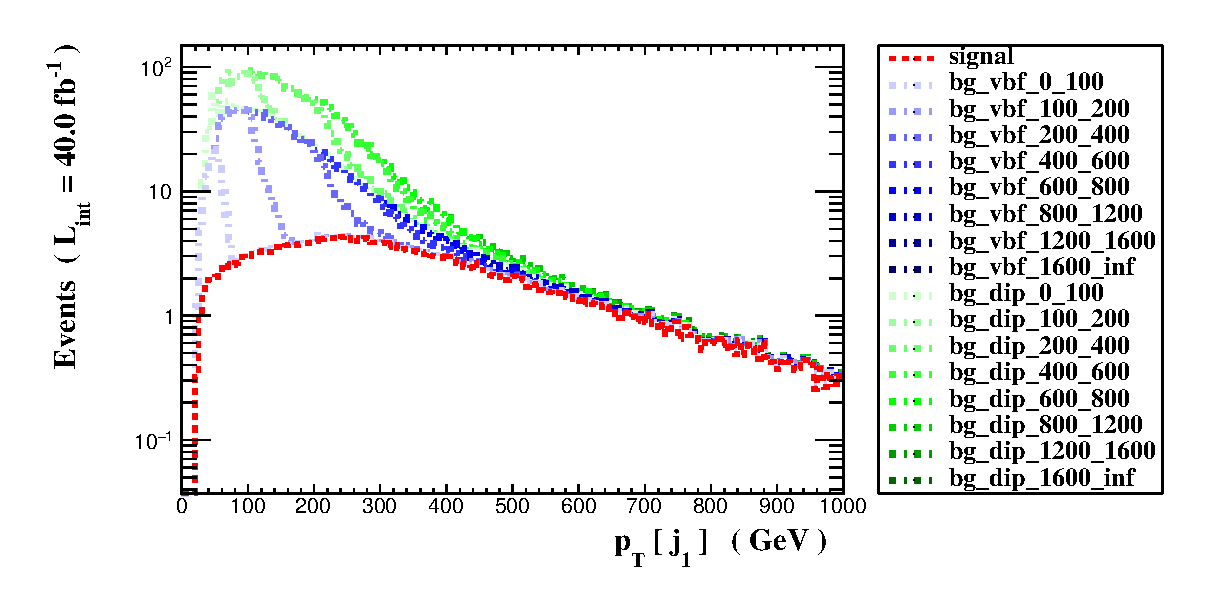
\includegraphics[scale=0.45]{selection_0.eps}\\
\caption{   }
  \end{center}
\end{figure}
      \newpage
\subsection{ Histogram 2}

\textbf{* Plot: ETA ( jets[1] ) }\\
   \begin{table}[H]
  \begin{center}
    \begin{tabular}{|m{23.0mm}|m{23.0mm}|m{18.0mm}|m{19.0mm}|m{19.0mm}|m{19.0mm}|m{19.0mm}|}
      \hline
      {\cellcolor{yellow}         Dataset}& {\cellcolor{yellow}         Integral}& {\cellcolor{yellow}         Entries per event}& {\cellcolor{yellow}         Mean}& {\cellcolor{yellow}         RMS}& {\cellcolor{yellow}         \% underflow}& {\cellcolor{yellow}         \% overflow}\\
      \hline
      {\cellcolor{white}         signal}& {\cellcolor{white}         405}& {\cellcolor{white}         1.0}& {\cellcolor{white}         1.93288}& {\cellcolor{white}         0.8878}& {\cellcolor{green}         0.0}& {\cellcolor{green}         0.0}\\
      \hline
      {\cellcolor{white}         bg\_vbf\_0\_100}& {\cellcolor{white}         102}& {\cellcolor{white}         1.0}& {\cellcolor{white}         3.69767}& {\cellcolor{white}         0.6913}& {\cellcolor{green}         0.0}& {\cellcolor{green}         0.0}\\
      \hline
      {\cellcolor{white}         bg\_vbf\_100\_200}& {\cellcolor{white}         477}& {\cellcolor{white}         1.0}& {\cellcolor{white}         3.05831}& {\cellcolor{white}         0.7484}& {\cellcolor{green}         0.0}& {\cellcolor{green}         0.0}\\
      \hline
      {\cellcolor{white}         bg\_vbf\_200\_400}& {\cellcolor{white}         573}& {\cellcolor{white}         1.0}& {\cellcolor{white}         2.48868}& {\cellcolor{white}         0.7253}& {\cellcolor{green}         0.0}& {\cellcolor{green}         0.0}\\
      \hline
      {\cellcolor{white}         bg\_vbf\_400\_600}& {\cellcolor{white}         136}& {\cellcolor{white}         1.0}& {\cellcolor{white}         2.07025}& {\cellcolor{white}         0.6598}& {\cellcolor{green}         0.0}& {\cellcolor{green}         0.0}\\
      \hline
      {\cellcolor{white}         bg\_vbf\_600\_800}& {\cellcolor{white}         23.8}& {\cellcolor{white}         1.0}& {\cellcolor{white}         1.96155}& {\cellcolor{white}         0.5638}& {\cellcolor{green}         0.0}& {\cellcolor{green}         0.0}\\
      \hline
      {\cellcolor{white}         bg\_vbf\_800\_1200}& {\cellcolor{white}         6.04}& {\cellcolor{white}         1.0}& {\cellcolor{white}         1.88259}& {\cellcolor{white}         0.4906}& {\cellcolor{green}         0.0}& {\cellcolor{green}         0.0}\\
      \hline
      {\cellcolor{white}         bg\_vbf\_1200\_1600}& {\cellcolor{white}         0.337}& {\cellcolor{white}         1.0}& {\cellcolor{white}         1.79038}& {\cellcolor{white}         0.437}& {\cellcolor{green}         0.0}& {\cellcolor{green}         0.0}\\
      \hline
      {\cellcolor{white}         bg\_vbf\_1600\_inf}& {\cellcolor{white}         0.0252}& {\cellcolor{white}         1.0}& {\cellcolor{white}         1.69945}& {\cellcolor{white}         0.4477}& {\cellcolor{green}         0.0}& {\cellcolor{green}         0.0}\\
      \hline
      {\cellcolor{white}         bg\_dip\_0\_100}& {\cellcolor{white}         117}& {\cellcolor{white}         1.0}& {\cellcolor{white}         3.61672}& {\cellcolor{white}         0.8533}& {\cellcolor{green}         0.0}& {\cellcolor{green}         0.0}\\
      \hline
      {\cellcolor{white}         bg\_dip\_100\_200}& {\cellcolor{white}         496}& {\cellcolor{white}         1.0}& {\cellcolor{white}         3.05543}& {\cellcolor{white}         0.9267}& {\cellcolor{green}         0.0}& {\cellcolor{green}         0.0}\\
      \hline
      {\cellcolor{white}         bg\_dip\_200\_400}& {\cellcolor{white}         814}& {\cellcolor{white}         1.0}& {\cellcolor{white}         2.39716}& {\cellcolor{white}         0.8274}& {\cellcolor{green}         0.0}& {\cellcolor{green}         0.0}\\
      \hline
      {\cellcolor{white}         bg\_dip\_400\_600}& {\cellcolor{white}         292}& {\cellcolor{white}         1.0}& {\cellcolor{white}         2.02025}& {\cellcolor{white}         0.7074}& {\cellcolor{green}         0.0}& {\cellcolor{green}         0.0}\\
      \hline
      {\cellcolor{white}         bg\_dip\_600\_800}& {\cellcolor{white}         44.6}& {\cellcolor{white}         1.0}& {\cellcolor{white}         1.92378}& {\cellcolor{white}         0.6381}& {\cellcolor{green}         0.0}& {\cellcolor{green}         0.0}\\
      \hline
      {\cellcolor{white}         bg\_dip\_800\_1200}& {\cellcolor{white}         10.9}& {\cellcolor{white}         1.0}& {\cellcolor{white}         1.80999}& {\cellcolor{white}         0.6146}& {\cellcolor{green}         0.0}& {\cellcolor{green}         0.0}\\
      \hline
      {\cellcolor{white}         bg\_dip\_1200\_1600}& {\cellcolor{white}         0.675}& {\cellcolor{white}         1.0}& {\cellcolor{white}         1.73565}& {\cellcolor{white}         0.5501}& {\cellcolor{green}         0.0}& {\cellcolor{green}         0.0}\\
      \hline
      {\cellcolor{white}         bg\_dip\_1600\_inf}& {\cellcolor{white}         0.0437}& {\cellcolor{white}         1.0}& {\cellcolor{white}         1.61899}& {\cellcolor{white}         0.6004}& {\cellcolor{green}         0.0}& {\cellcolor{green}         0.0}\\
\hline
    \end{tabular}
  \end{center}
\end{table}

\begin{figure}[H]
  \begin{center}
    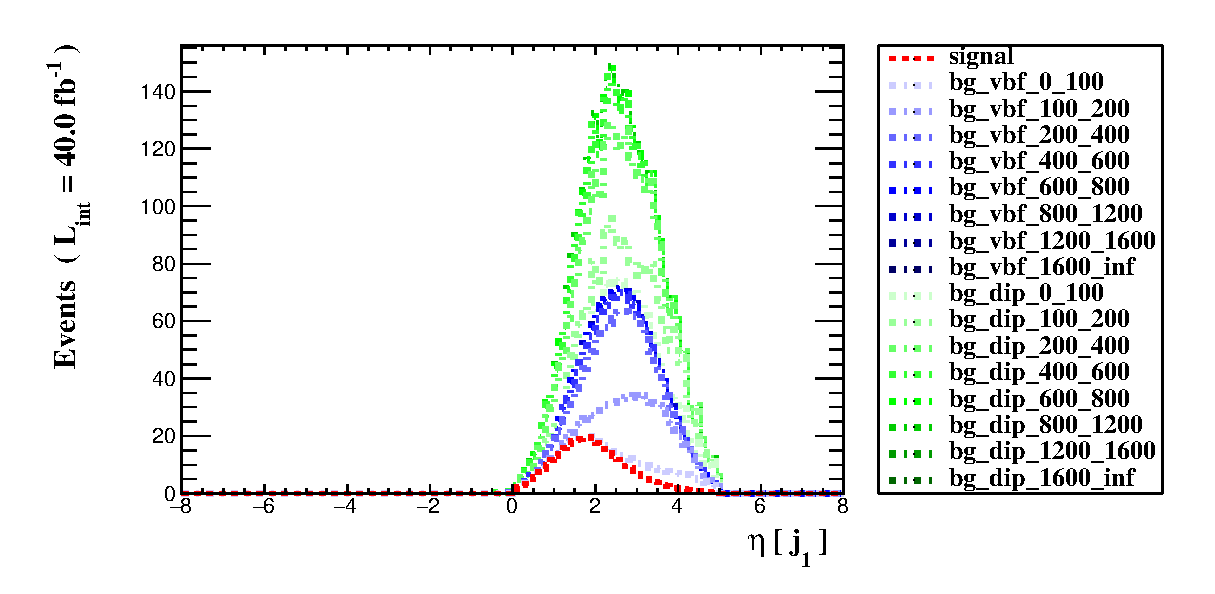
\includegraphics[scale=0.45]{selection_1.eps}\\
\caption{   }
  \end{center}
\end{figure}
      \newpage
\subsection{ Histogram 3}

\textbf{* Plot: PHI ( jets[1] ) }\\
   \begin{table}[H]
  \begin{center}
    \begin{tabular}{|m{23.0mm}|m{23.0mm}|m{18.0mm}|m{19.0mm}|m{19.0mm}|m{19.0mm}|m{19.0mm}|}
      \hline
      {\cellcolor{yellow}         Dataset}& {\cellcolor{yellow}         Integral}& {\cellcolor{yellow}         Entries per event}& {\cellcolor{yellow}         Mean}& {\cellcolor{yellow}         RMS}& {\cellcolor{yellow}         \% underflow}& {\cellcolor{yellow}         \% overflow}\\
      \hline
      {\cellcolor{white}         signal}& {\cellcolor{white}         405}& {\cellcolor{white}         1.0}& {\cellcolor{white}         -0.000461567}& {\cellcolor{white}         1.813}& {\cellcolor{green}         0.0}& {\cellcolor{green}         0.0}\\
      \hline
      {\cellcolor{white}         bg\_vbf\_0\_100}& {\cellcolor{white}         102}& {\cellcolor{white}         1.0}& {\cellcolor{white}         -0.00381425}& {\cellcolor{white}         1.809}& {\cellcolor{green}         0.0}& {\cellcolor{green}         0.0}\\
      \hline
      {\cellcolor{white}         bg\_vbf\_100\_200}& {\cellcolor{white}         477}& {\cellcolor{white}         1.0}& {\cellcolor{white}         -0.00399372}& {\cellcolor{white}         1.815}& {\cellcolor{green}         0.0}& {\cellcolor{green}         0.0}\\
      \hline
      {\cellcolor{white}         bg\_vbf\_200\_400}& {\cellcolor{white}         573}& {\cellcolor{white}         1.0}& {\cellcolor{white}         -0.000180864}& {\cellcolor{white}         1.812}& {\cellcolor{green}         0.0}& {\cellcolor{green}         0.0}\\
      \hline
      {\cellcolor{white}         bg\_vbf\_400\_600}& {\cellcolor{white}         136}& {\cellcolor{white}         1.0}& {\cellcolor{white}         -0.00076842}& {\cellcolor{white}         1.812}& {\cellcolor{green}         0.0}& {\cellcolor{green}         0.0}\\
      \hline
      {\cellcolor{white}         bg\_vbf\_600\_800}& {\cellcolor{white}         23.8}& {\cellcolor{white}         1.0}& {\cellcolor{white}         0.00932615}& {\cellcolor{white}         1.812}& {\cellcolor{green}         0.0}& {\cellcolor{green}         0.0}\\
      \hline
      {\cellcolor{white}         bg\_vbf\_800\_1200}& {\cellcolor{white}         6.04}& {\cellcolor{white}         1.0}& {\cellcolor{white}         -0.00383047}& {\cellcolor{white}         1.813}& {\cellcolor{green}         0.0}& {\cellcolor{green}         0.0}\\
      \hline
      {\cellcolor{white}         bg\_vbf\_1200\_1600}& {\cellcolor{white}         0.337}& {\cellcolor{white}         1.0}& {\cellcolor{white}         0.0192996}& {\cellcolor{white}         1.809}& {\cellcolor{green}         0.0}& {\cellcolor{green}         0.0}\\
      \hline
      {\cellcolor{white}         bg\_vbf\_1600\_inf}& {\cellcolor{white}         0.0252}& {\cellcolor{white}         1.0}& {\cellcolor{white}         -0.0612997}& {\cellcolor{white}         1.785}& {\cellcolor{green}         0.0}& {\cellcolor{green}         0.0}\\
      \hline
      {\cellcolor{white}         bg\_dip\_0\_100}& {\cellcolor{white}         117}& {\cellcolor{white}         1.0}& {\cellcolor{white}         0.131552}& {\cellcolor{white}         1.932}& {\cellcolor{green}         0.0}& {\cellcolor{green}         0.0}\\
      \hline
      {\cellcolor{white}         bg\_dip\_100\_200}& {\cellcolor{white}         496}& {\cellcolor{white}         1.0}& {\cellcolor{white}         -0.0494161}& {\cellcolor{white}         1.808}& {\cellcolor{green}         0.0}& {\cellcolor{green}         0.0}\\
      \hline
      {\cellcolor{white}         bg\_dip\_200\_400}& {\cellcolor{white}         814}& {\cellcolor{white}         1.0}& {\cellcolor{white}         -0.0325304}& {\cellcolor{white}         1.8}& {\cellcolor{green}         0.0}& {\cellcolor{green}         0.0}\\
      \hline
      {\cellcolor{white}         bg\_dip\_400\_600}& {\cellcolor{white}         292}& {\cellcolor{white}         1.0}& {\cellcolor{white}         -0.0169474}& {\cellcolor{white}         1.802}& {\cellcolor{green}         0.0}& {\cellcolor{green}         0.0}\\
      \hline
      {\cellcolor{white}         bg\_dip\_600\_800}& {\cellcolor{white}         44.6}& {\cellcolor{white}         1.0}& {\cellcolor{white}         -0.0041996}& {\cellcolor{white}         1.819}& {\cellcolor{green}         0.0}& {\cellcolor{green}         0.0}\\
      \hline
      {\cellcolor{white}         bg\_dip\_800\_1200}& {\cellcolor{white}         10.9}& {\cellcolor{white}         1.0}& {\cellcolor{white}         0.0287461}& {\cellcolor{white}         1.813}& {\cellcolor{green}         0.0}& {\cellcolor{green}         0.0}\\
      \hline
      {\cellcolor{white}         bg\_dip\_1200\_1600}& {\cellcolor{white}         0.675}& {\cellcolor{white}         1.0}& {\cellcolor{white}         -0.111858}& {\cellcolor{white}         1.79}& {\cellcolor{green}         0.0}& {\cellcolor{green}         0.0}\\
      \hline
      {\cellcolor{white}         bg\_dip\_1600\_inf}& {\cellcolor{white}         0.0437}& {\cellcolor{white}         1.0}& {\cellcolor{white}         -0.0242244}& {\cellcolor{white}         1.737}& {\cellcolor{green}         0.0}& {\cellcolor{green}         0.0}\\
\hline
    \end{tabular}
  \end{center}
\end{table}

\begin{figure}[H]
  \begin{center}
    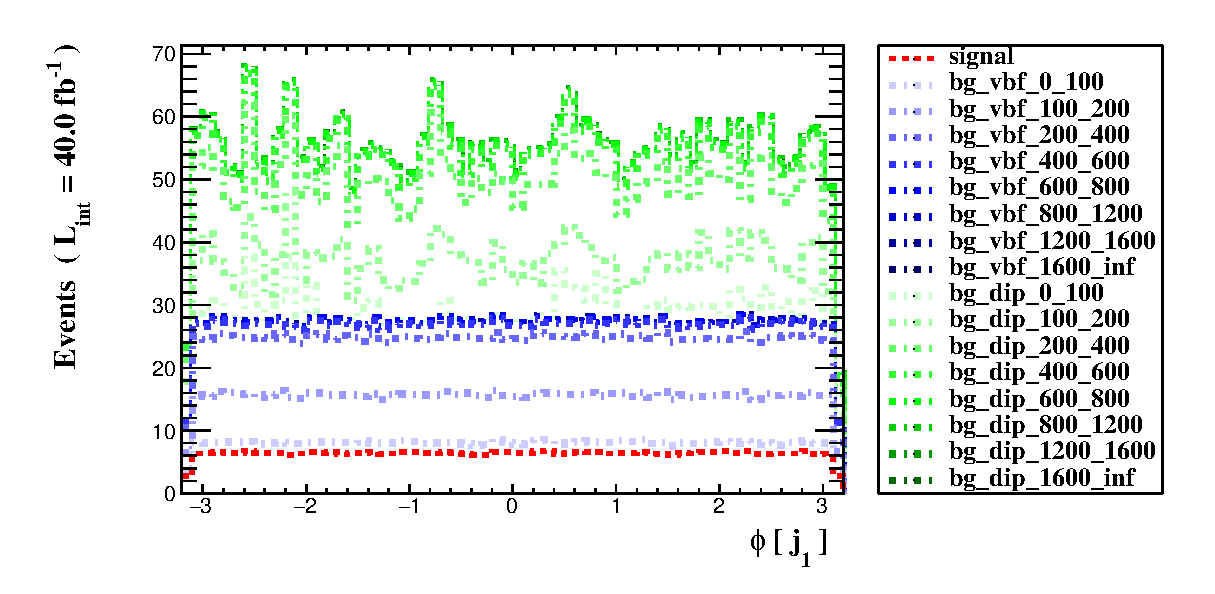
\includegraphics[scale=0.45]{selection_2.eps}\\
\caption{   }
  \end{center}
\end{figure}
      \newpage
\subsection{ Histogram 4}

\textbf{* Plot: PT ( jets[2] ) }\\
   \begin{table}[H]
  \begin{center}
    \begin{tabular}{|m{23.0mm}|m{23.0mm}|m{18.0mm}|m{19.0mm}|m{19.0mm}|m{19.0mm}|m{19.0mm}|}
      \hline
      {\cellcolor{yellow}         Dataset}& {\cellcolor{yellow}         Integral}& {\cellcolor{yellow}         Entries per event}& {\cellcolor{yellow}         Mean}& {\cellcolor{yellow}         RMS}& {\cellcolor{yellow}         \% underflow}& {\cellcolor{yellow}         \% overflow}\\
      \hline
      {\cellcolor{white}         signal}& {\cellcolor{white}         405}& {\cellcolor{white}         1.0}& {\cellcolor{white}         118.962}& {\cellcolor{white}         84.1}& {\cellcolor{green}         0.0}& {\cellcolor{green}         0.2323}\\
      \hline
      {\cellcolor{white}         bg\_vbf\_0\_100}& {\cellcolor{white}         102}& {\cellcolor{white}         1.0}& {\cellcolor{white}         32.1093}& {\cellcolor{white}         7.26}& {\cellcolor{green}         0.0}& {\cellcolor{green}         0.0}\\
      \hline
      {\cellcolor{white}         bg\_vbf\_100\_200}& {\cellcolor{white}         477}& {\cellcolor{white}         1.0}& {\cellcolor{white}         59.3482}& {\cellcolor{white}         16.86}& {\cellcolor{green}         0.0}& {\cellcolor{green}         0.0}\\
      \hline
      {\cellcolor{white}         bg\_vbf\_200\_400}& {\cellcolor{white}         573}& {\cellcolor{white}         1.0}& {\cellcolor{white}         115.402}& {\cellcolor{white}         33.11}& {\cellcolor{green}         0.0}& {\cellcolor{green}         0.0}\\
      \hline
      {\cellcolor{white}         bg\_vbf\_400\_600}& {\cellcolor{white}         136}& {\cellcolor{white}         1.0}& {\cellcolor{white}         195.78}& {\cellcolor{white}         46.92}& {\cellcolor{green}         0.0}& {\cellcolor{green}         0.0}\\
      \hline
      {\cellcolor{white}         bg\_vbf\_600\_800}& {\cellcolor{white}         23.8}& {\cellcolor{white}         1.0}& {\cellcolor{white}         279.817}& {\cellcolor{white}         70.52}& {\cellcolor{green}         0.0}& {\cellcolor{green}         0.0}\\
      \hline
      {\cellcolor{white}         bg\_vbf\_800\_1200}& {\cellcolor{white}         6.04}& {\cellcolor{white}         1.0}& {\cellcolor{white}         381.023}& {\cellcolor{white}         107.6}& {\cellcolor{orange}         0.0}& {\cellcolor{orange}         8.421}\\
      \hline
      {\cellcolor{white}         bg\_vbf\_1200\_1600}& {\cellcolor{white}         0.337}& {\cellcolor{white}         1.0}& {\cellcolor{white}         548.791}& {\cellcolor{white}         166.3}& {\cellcolor{red}         0.0}& {\cellcolor{red}         78.99}\\
      \hline
      {\cellcolor{white}         bg\_vbf\_1600\_inf}& {\cellcolor{white}         0.0252}& {\cellcolor{white}         1.0}& {\cellcolor{white}         704.575}& {\cellcolor{white}         256.7}& {\cellcolor{red}         0.0}& {\cellcolor{red}         83.13}\\
      \hline
      {\cellcolor{white}         bg\_dip\_0\_100}& {\cellcolor{white}         117}& {\cellcolor{white}         1.0}& {\cellcolor{white}         32.1082}& {\cellcolor{white}         6.852}& {\cellcolor{green}         0.0}& {\cellcolor{green}         0.0}\\
      \hline
      {\cellcolor{white}         bg\_dip\_100\_200}& {\cellcolor{white}         496}& {\cellcolor{white}         1.0}& {\cellcolor{white}         58.8617}& {\cellcolor{white}         17.59}& {\cellcolor{green}         0.0}& {\cellcolor{green}         0.0}\\
      \hline
      {\cellcolor{white}         bg\_dip\_200\_400}& {\cellcolor{white}         814}& {\cellcolor{white}         1.0}& {\cellcolor{white}         119.32}& {\cellcolor{white}         37.13}& {\cellcolor{green}         0.0}& {\cellcolor{green}         0.0}\\
      \hline
      {\cellcolor{white}         bg\_dip\_400\_600}& {\cellcolor{white}         292}& {\cellcolor{white}         1.0}& {\cellcolor{white}         196.391}& {\cellcolor{white}         49.4}& {\cellcolor{green}         0.0}& {\cellcolor{green}         0.0}\\
      \hline
      {\cellcolor{white}         bg\_dip\_600\_800}& {\cellcolor{white}         44.6}& {\cellcolor{white}         1.0}& {\cellcolor{white}         279.332}& {\cellcolor{white}         79.47}& {\cellcolor{green}         0.0}& {\cellcolor{green}         0.0}\\
      \hline
      {\cellcolor{white}         bg\_dip\_800\_1200}& {\cellcolor{white}         10.9}& {\cellcolor{white}         1.0}& {\cellcolor{white}         370.05}& {\cellcolor{white}         134.1}& {\cellcolor{orange}         0.0}& {\cellcolor{orange}         8.548}\\
      \hline
      {\cellcolor{white}         bg\_dip\_1200\_1600}& {\cellcolor{white}         0.675}& {\cellcolor{white}         1.0}& {\cellcolor{white}         537.054}& {\cellcolor{white}         199.7}& {\cellcolor{red}         0.0}& {\cellcolor{red}         81.48}\\
      \hline
      {\cellcolor{white}         bg\_dip\_1600\_inf}& {\cellcolor{white}         0.0437}& {\cellcolor{white}         1.0}& {\cellcolor{white}         699.472}& {\cellcolor{white}         304.3}& {\cellcolor{red}         0.0}& {\cellcolor{red}         82.64}\\
\hline
    \end{tabular}
  \end{center}
\end{table}

\begin{figure}[H]
  \begin{center}
    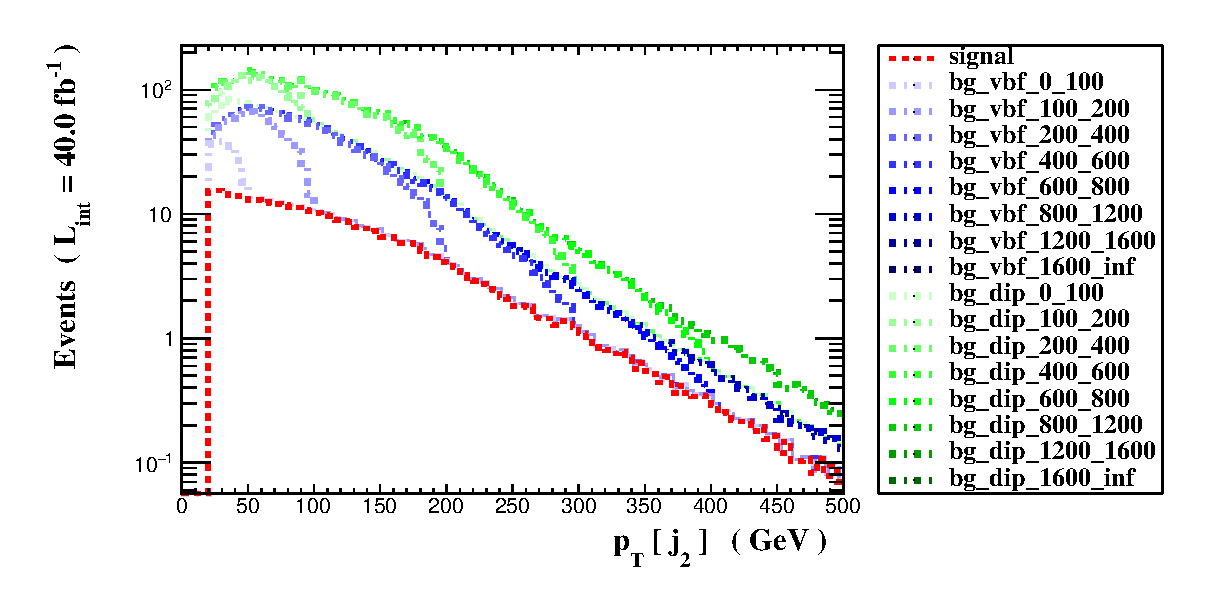
\includegraphics[scale=0.45]{selection_3.eps}\\
\caption{   }
  \end{center}
\end{figure}
      \newpage
\subsection{ Histogram 5}

\textbf{* Plot: ETA ( jets[2] ) }\\
   \begin{table}[H]
  \begin{center}
    \begin{tabular}{|m{23.0mm}|m{23.0mm}|m{18.0mm}|m{19.0mm}|m{19.0mm}|m{19.0mm}|m{19.0mm}|}
      \hline
      {\cellcolor{yellow}         Dataset}& {\cellcolor{yellow}         Integral}& {\cellcolor{yellow}         Entries per event}& {\cellcolor{yellow}         Mean}& {\cellcolor{yellow}         RMS}& {\cellcolor{yellow}         \% underflow}& {\cellcolor{yellow}         \% overflow}\\
      \hline
      {\cellcolor{white}         signal}& {\cellcolor{white}         405}& {\cellcolor{white}         1.0}& {\cellcolor{white}         -3.00573}& {\cellcolor{white}         0.8372}& {\cellcolor{green}         0.0}& {\cellcolor{green}         0.0}\\
      \hline
      {\cellcolor{white}         bg\_vbf\_0\_100}& {\cellcolor{white}         102}& {\cellcolor{white}         1.0}& {\cellcolor{white}         -3.87669}& {\cellcolor{white}         0.6852}& {\cellcolor{green}         0.0}& {\cellcolor{green}         0.0}\\
      \hline
      {\cellcolor{white}         bg\_vbf\_100\_200}& {\cellcolor{white}         477}& {\cellcolor{white}         1.0}& {\cellcolor{white}         -3.34195}& {\cellcolor{white}         0.7753}& {\cellcolor{green}         0.0}& {\cellcolor{green}         0.0}\\
      \hline
      {\cellcolor{white}         bg\_vbf\_200\_400}& {\cellcolor{white}         573}& {\cellcolor{white}         1.0}& {\cellcolor{white}         -2.76309}& {\cellcolor{white}         0.7681}& {\cellcolor{green}         0.0}& {\cellcolor{green}         0.0}\\
      \hline
      {\cellcolor{white}         bg\_vbf\_400\_600}& {\cellcolor{white}         136}& {\cellcolor{white}         1.0}& {\cellcolor{white}         -2.34591}& {\cellcolor{white}         0.6955}& {\cellcolor{green}         0.0}& {\cellcolor{green}         0.0}\\
      \hline
      {\cellcolor{white}         bg\_vbf\_600\_800}& {\cellcolor{white}         23.8}& {\cellcolor{white}         1.0}& {\cellcolor{white}         -2.26091}& {\cellcolor{white}         0.5995}& {\cellcolor{green}         0.0}& {\cellcolor{green}         0.0}\\
      \hline
      {\cellcolor{white}         bg\_vbf\_800\_1200}& {\cellcolor{white}         6.04}& {\cellcolor{white}         1.0}& {\cellcolor{white}         -2.19432}& {\cellcolor{white}         0.5325}& {\cellcolor{green}         0.0}& {\cellcolor{green}         0.0}\\
      \hline
      {\cellcolor{white}         bg\_vbf\_1200\_1600}& {\cellcolor{white}         0.337}& {\cellcolor{white}         1.0}& {\cellcolor{white}         -2.14009}& {\cellcolor{white}         0.4985}& {\cellcolor{green}         0.0}& {\cellcolor{green}         0.0}\\
      \hline
      {\cellcolor{white}         bg\_vbf\_1600\_inf}& {\cellcolor{white}         0.0252}& {\cellcolor{white}         1.0}& {\cellcolor{white}         -2.14792}& {\cellcolor{white}         0.5185}& {\cellcolor{green}         0.0}& {\cellcolor{green}         0.0}\\
      \hline
      {\cellcolor{white}         bg\_dip\_0\_100}& {\cellcolor{white}         117}& {\cellcolor{white}         1.0}& {\cellcolor{white}         -3.69603}& {\cellcolor{white}         0.8703}& {\cellcolor{green}         0.0}& {\cellcolor{green}         0.0}\\
      \hline
      {\cellcolor{white}         bg\_dip\_100\_200}& {\cellcolor{white}         496}& {\cellcolor{white}         1.0}& {\cellcolor{white}         -3.05582}& {\cellcolor{white}         0.9476}& {\cellcolor{green}         0.0}& {\cellcolor{green}         0.0}\\
      \hline
      {\cellcolor{white}         bg\_dip\_200\_400}& {\cellcolor{white}         814}& {\cellcolor{white}         1.0}& {\cellcolor{white}         -2.42149}& {\cellcolor{white}         0.9066}& {\cellcolor{green}         0.0}& {\cellcolor{green}         0.0}\\
      \hline
      {\cellcolor{white}         bg\_dip\_400\_600}& {\cellcolor{white}         292}& {\cellcolor{white}         1.0}& {\cellcolor{white}         -2.06643}& {\cellcolor{white}         0.7781}& {\cellcolor{green}         0.0}& {\cellcolor{green}         0.0}\\
      \hline
      {\cellcolor{white}         bg\_dip\_600\_800}& {\cellcolor{white}         44.6}& {\cellcolor{white}         1.0}& {\cellcolor{white}         -2.09025}& {\cellcolor{white}         0.708}& {\cellcolor{green}         0.0}& {\cellcolor{green}         0.0}\\
      \hline
      {\cellcolor{white}         bg\_dip\_800\_1200}& {\cellcolor{white}         10.9}& {\cellcolor{white}         1.0}& {\cellcolor{white}         -2.14791}& {\cellcolor{white}         0.7068}& {\cellcolor{green}         0.0}& {\cellcolor{green}         0.0}\\
      \hline
      {\cellcolor{white}         bg\_dip\_1200\_1600}& {\cellcolor{white}         0.675}& {\cellcolor{white}         1.0}& {\cellcolor{white}         -2.13001}& {\cellcolor{white}         0.6727}& {\cellcolor{green}         0.0}& {\cellcolor{green}         0.0}\\
      \hline
      {\cellcolor{white}         bg\_dip\_1600\_inf}& {\cellcolor{white}         0.0437}& {\cellcolor{white}         1.0}& {\cellcolor{white}         -2.20017}& {\cellcolor{white}         0.7261}& {\cellcolor{green}         0.0}& {\cellcolor{green}         0.0}\\
\hline
    \end{tabular}
  \end{center}
\end{table}

\begin{figure}[H]
  \begin{center}
    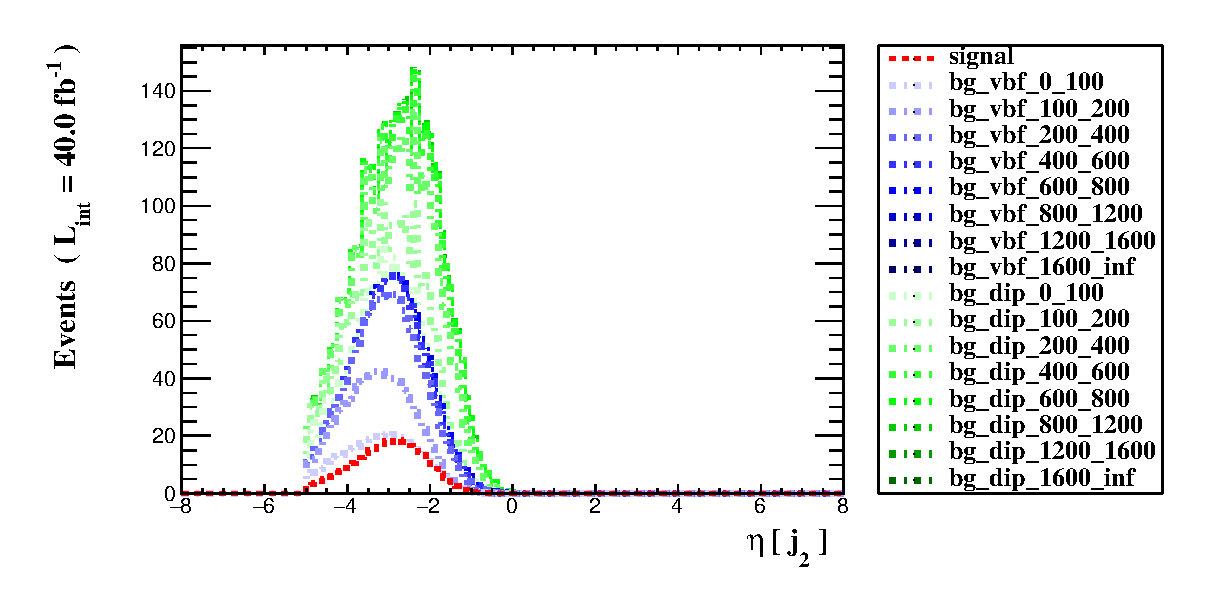
\includegraphics[scale=0.45]{selection_4.eps}\\
\caption{   }
  \end{center}
\end{figure}
      \newpage
\subsection{ Histogram 6}

\textbf{* Plot: PHI ( jets[2] ) }\\
   \begin{table}[H]
  \begin{center}
    \begin{tabular}{|m{23.0mm}|m{23.0mm}|m{18.0mm}|m{19.0mm}|m{19.0mm}|m{19.0mm}|m{19.0mm}|}
      \hline
      {\cellcolor{yellow}         Dataset}& {\cellcolor{yellow}         Integral}& {\cellcolor{yellow}         Entries per event}& {\cellcolor{yellow}         Mean}& {\cellcolor{yellow}         RMS}& {\cellcolor{yellow}         \% underflow}& {\cellcolor{yellow}         \% overflow}\\
      \hline
      {\cellcolor{white}         signal}& {\cellcolor{white}         405}& {\cellcolor{white}         1.0}& {\cellcolor{white}         -0.00526342}& {\cellcolor{white}         1.814}& {\cellcolor{green}         0.0}& {\cellcolor{green}         0.0}\\
      \hline
      {\cellcolor{white}         bg\_vbf\_0\_100}& {\cellcolor{white}         102}& {\cellcolor{white}         1.0}& {\cellcolor{white}         -0.0109881}& {\cellcolor{white}         1.822}& {\cellcolor{green}         0.0}& {\cellcolor{green}         0.0}\\
      \hline
      {\cellcolor{white}         bg\_vbf\_100\_200}& {\cellcolor{white}         477}& {\cellcolor{white}         1.0}& {\cellcolor{white}         0.00648616}& {\cellcolor{white}         1.818}& {\cellcolor{green}         0.0}& {\cellcolor{green}         0.0}\\
      \hline
      {\cellcolor{white}         bg\_vbf\_200\_400}& {\cellcolor{white}         573}& {\cellcolor{white}         1.0}& {\cellcolor{white}         -0.000152277}& {\cellcolor{white}         1.815}& {\cellcolor{green}         0.0}& {\cellcolor{green}         0.0}\\
      \hline
      {\cellcolor{white}         bg\_vbf\_400\_600}& {\cellcolor{white}         136}& {\cellcolor{white}         1.0}& {\cellcolor{white}         -0.00184318}& {\cellcolor{white}         1.815}& {\cellcolor{green}         0.0}& {\cellcolor{green}         0.0}\\
      \hline
      {\cellcolor{white}         bg\_vbf\_600\_800}& {\cellcolor{white}         23.8}& {\cellcolor{white}         1.0}& {\cellcolor{white}         -0.00298582}& {\cellcolor{white}         1.817}& {\cellcolor{green}         0.0}& {\cellcolor{green}         0.0}\\
      \hline
      {\cellcolor{white}         bg\_vbf\_800\_1200}& {\cellcolor{white}         6.04}& {\cellcolor{white}         1.0}& {\cellcolor{white}         -0.0150365}& {\cellcolor{white}         1.818}& {\cellcolor{green}         0.0}& {\cellcolor{green}         0.0}\\
      \hline
      {\cellcolor{white}         bg\_vbf\_1200\_1600}& {\cellcolor{white}         0.337}& {\cellcolor{white}         1.0}& {\cellcolor{white}         -0.00539569}& {\cellcolor{white}         1.822}& {\cellcolor{green}         0.0}& {\cellcolor{green}         0.0}\\
      \hline
      {\cellcolor{white}         bg\_vbf\_1600\_inf}& {\cellcolor{white}         0.0252}& {\cellcolor{white}         1.0}& {\cellcolor{white}         0.0399503}& {\cellcolor{white}         1.79}& {\cellcolor{green}         0.0}& {\cellcolor{green}         0.0}\\
      \hline
      {\cellcolor{white}         bg\_dip\_0\_100}& {\cellcolor{white}         117}& {\cellcolor{white}         1.0}& {\cellcolor{white}         -0.382442}& {\cellcolor{white}         1.517}& {\cellcolor{green}         0.0}& {\cellcolor{green}         0.0}\\
      \hline
      {\cellcolor{white}         bg\_dip\_100\_200}& {\cellcolor{white}         496}& {\cellcolor{white}         1.0}& {\cellcolor{white}         0.0518113}& {\cellcolor{white}         1.834}& {\cellcolor{green}         0.0}& {\cellcolor{green}         0.0}\\
      \hline
      {\cellcolor{white}         bg\_dip\_200\_400}& {\cellcolor{white}         814}& {\cellcolor{white}         1.0}& {\cellcolor{white}         -0.013668}& {\cellcolor{white}         1.825}& {\cellcolor{green}         0.0}& {\cellcolor{green}         0.0}\\
      \hline
      {\cellcolor{white}         bg\_dip\_400\_600}& {\cellcolor{white}         292}& {\cellcolor{white}         1.0}& {\cellcolor{white}         -0.0161945}& {\cellcolor{white}         1.826}& {\cellcolor{green}         0.0}& {\cellcolor{green}         0.0}\\
      \hline
      {\cellcolor{white}         bg\_dip\_600\_800}& {\cellcolor{white}         44.6}& {\cellcolor{white}         1.0}& {\cellcolor{white}         -0.0181903}& {\cellcolor{white}         1.811}& {\cellcolor{green}         0.0}& {\cellcolor{green}         0.0}\\
      \hline
      {\cellcolor{white}         bg\_dip\_800\_1200}& {\cellcolor{white}         10.9}& {\cellcolor{white}         1.0}& {\cellcolor{white}         -0.0153119}& {\cellcolor{white}         1.817}& {\cellcolor{green}         0.0}& {\cellcolor{green}         0.0}\\
      \hline
      {\cellcolor{white}         bg\_dip\_1200\_1600}& {\cellcolor{white}         0.675}& {\cellcolor{white}         1.0}& {\cellcolor{white}         0.0739514}& {\cellcolor{white}         1.823}& {\cellcolor{green}         0.0}& {\cellcolor{green}         0.0}\\
      \hline
      {\cellcolor{white}         bg\_dip\_1600\_inf}& {\cellcolor{white}         0.0437}& {\cellcolor{white}         1.0}& {\cellcolor{white}         -0.174818}& {\cellcolor{white}         1.849}& {\cellcolor{green}         0.0}& {\cellcolor{green}         0.0}\\
\hline
    \end{tabular}
  \end{center}
\end{table}

\begin{figure}[H]
  \begin{center}
    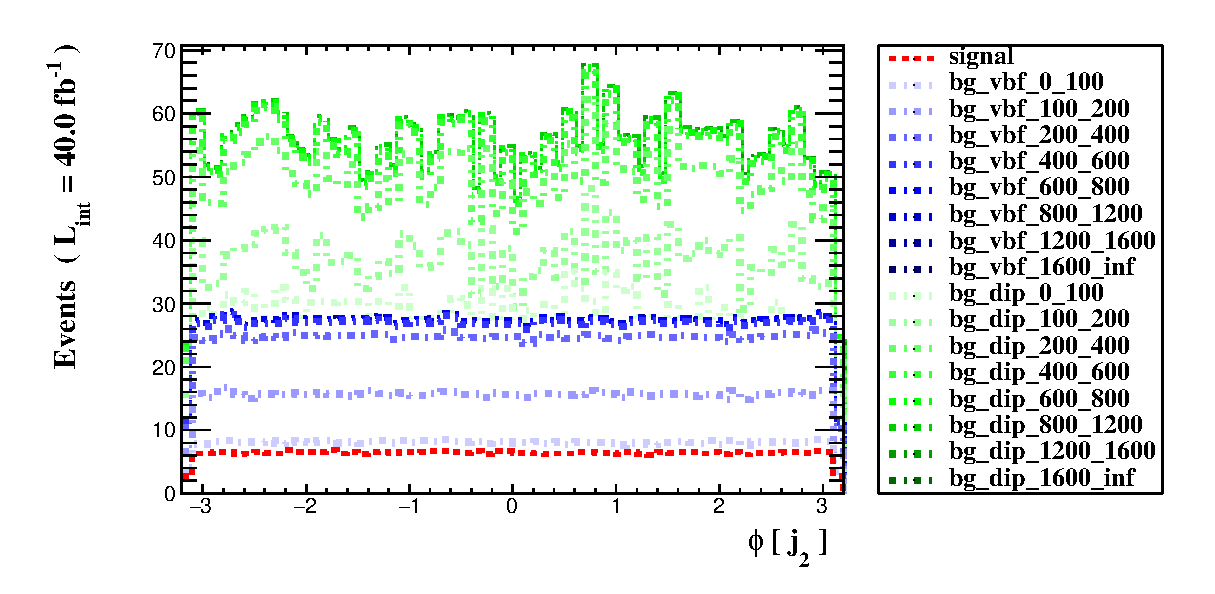
\includegraphics[scale=0.45]{selection_5.eps}\\
\caption{   }
  \end{center}
\end{figure}
      \newpage
\subsection{ Histogram 7}

\textbf{* Plot: DELTAR ( jets[1] , jets[2] ) }\\
   \begin{table}[H]
  \begin{center}
    \begin{tabular}{|m{23.0mm}|m{23.0mm}|m{18.0mm}|m{19.0mm}|m{19.0mm}|m{19.0mm}|m{19.0mm}|}
      \hline
      {\cellcolor{yellow}         Dataset}& {\cellcolor{yellow}         Integral}& {\cellcolor{yellow}         Entries per event}& {\cellcolor{yellow}         Mean}& {\cellcolor{yellow}         RMS}& {\cellcolor{yellow}         \% underflow}& {\cellcolor{yellow}         \% overflow}\\
      \hline
      {\cellcolor{white}         signal}& {\cellcolor{white}         405}& {\cellcolor{white}         1.0}& {\cellcolor{white}         5.27638}& {\cellcolor{white}         1.111}& {\cellcolor{green}         0.0}& {\cellcolor{green}         0.0}\\
      \hline
      {\cellcolor{white}         bg\_vbf\_0\_100}& {\cellcolor{white}         102}& {\cellcolor{white}         1.0}& {\cellcolor{white}         7.95218}& {\cellcolor{white}         0.591}& {\cellcolor{green}         0.0}& {\cellcolor{green}         0.0}\\
      \hline
      {\cellcolor{white}         bg\_vbf\_100\_200}& {\cellcolor{white}         477}& {\cellcolor{white}         1.0}& {\cellcolor{white}         6.93039}& {\cellcolor{white}         0.6173}& {\cellcolor{green}         0.0}& {\cellcolor{green}         0.0}\\
      \hline
      {\cellcolor{white}         bg\_vbf\_200\_400}& {\cellcolor{white}         573}& {\cellcolor{white}         1.0}& {\cellcolor{white}         5.94197}& {\cellcolor{white}         0.6418}& {\cellcolor{green}         0.0}& {\cellcolor{green}         0.0}\\
      \hline
      {\cellcolor{white}         bg\_vbf\_400\_600}& {\cellcolor{white}         136}& {\cellcolor{white}         1.0}& {\cellcolor{white}         5.24308}& {\cellcolor{white}         0.5412}& {\cellcolor{green}         0.0}& {\cellcolor{green}         0.0}\\
      \hline
      {\cellcolor{white}         bg\_vbf\_600\_800}& {\cellcolor{white}         23.8}& {\cellcolor{white}         1.0}& {\cellcolor{white}         5.09234}& {\cellcolor{white}         0.4485}& {\cellcolor{green}         0.0}& {\cellcolor{green}         0.0}\\
      \hline
      {\cellcolor{white}         bg\_vbf\_800\_1200}& {\cellcolor{white}         6.04}& {\cellcolor{white}         1.0}& {\cellcolor{white}         4.98571}& {\cellcolor{white}         0.3741}& {\cellcolor{green}         0.0}& {\cellcolor{green}         0.0}\\
      \hline
      {\cellcolor{white}         bg\_vbf\_1200\_1600}& {\cellcolor{white}         0.337}& {\cellcolor{white}         1.0}& {\cellcolor{white}         4.88302}& {\cellcolor{white}         0.3}& {\cellcolor{green}         0.0}& {\cellcolor{green}         0.0}\\
      \hline
      {\cellcolor{white}         bg\_vbf\_1600\_inf}& {\cellcolor{white}         0.0252}& {\cellcolor{white}         1.0}& {\cellcolor{white}         4.82191}& {\cellcolor{white}         0.2795}& {\cellcolor{green}         0.0}& {\cellcolor{green}         0.0}\\
      \hline
      {\cellcolor{white}         bg\_dip\_0\_100}& {\cellcolor{white}         117}& {\cellcolor{white}         1.0}& {\cellcolor{white}         7.74752}& {\cellcolor{white}         0.3267}& {\cellcolor{green}         0.0}& {\cellcolor{green}         0.0}\\
      \hline
      {\cellcolor{white}         bg\_dip\_100\_200}& {\cellcolor{white}         496}& {\cellcolor{white}         1.0}& {\cellcolor{white}         6.66929}& {\cellcolor{white}         0.4759}& {\cellcolor{green}         0.0}& {\cellcolor{green}         0.0}\\
      \hline
      {\cellcolor{white}         bg\_dip\_200\_400}& {\cellcolor{white}         814}& {\cellcolor{white}         1.0}& {\cellcolor{white}         5.59206}& {\cellcolor{white}         0.4871}& {\cellcolor{green}         0.0}& {\cellcolor{green}         0.0}\\
      \hline
      {\cellcolor{white}         bg\_dip\_400\_600}& {\cellcolor{white}         292}& {\cellcolor{white}         1.0}& {\cellcolor{white}         5.01265}& {\cellcolor{white}         0.3721}& {\cellcolor{green}         0.0}& {\cellcolor{green}         0.0}\\
      \hline
      {\cellcolor{white}         bg\_dip\_600\_800}& {\cellcolor{white}         44.6}& {\cellcolor{white}         1.0}& {\cellcolor{white}         4.9591}& {\cellcolor{white}         0.329}& {\cellcolor{green}         0.0}& {\cellcolor{green}         0.0}\\
      \hline
      {\cellcolor{white}         bg\_dip\_800\_1200}& {\cellcolor{white}         10.9}& {\cellcolor{white}         1.0}& {\cellcolor{white}         4.90662}& {\cellcolor{white}         0.3104}& {\cellcolor{green}         0.0}& {\cellcolor{green}         0.0}\\
      \hline
      {\cellcolor{white}         bg\_dip\_1200\_1600}& {\cellcolor{white}         0.675}& {\cellcolor{white}         1.0}& {\cellcolor{white}         4.82935}& {\cellcolor{white}         0.2943}& {\cellcolor{green}         0.0}& {\cellcolor{green}         0.0}\\
      \hline
      {\cellcolor{white}         bg\_dip\_1600\_inf}& {\cellcolor{white}         0.0437}& {\cellcolor{white}         1.0}& {\cellcolor{white}         4.78152}& {\cellcolor{white}         0.2814}& {\cellcolor{green}         0.0}& {\cellcolor{green}         0.0}\\
\hline
    \end{tabular}
  \end{center}
\end{table}

\begin{figure}[H]
  \begin{center}
    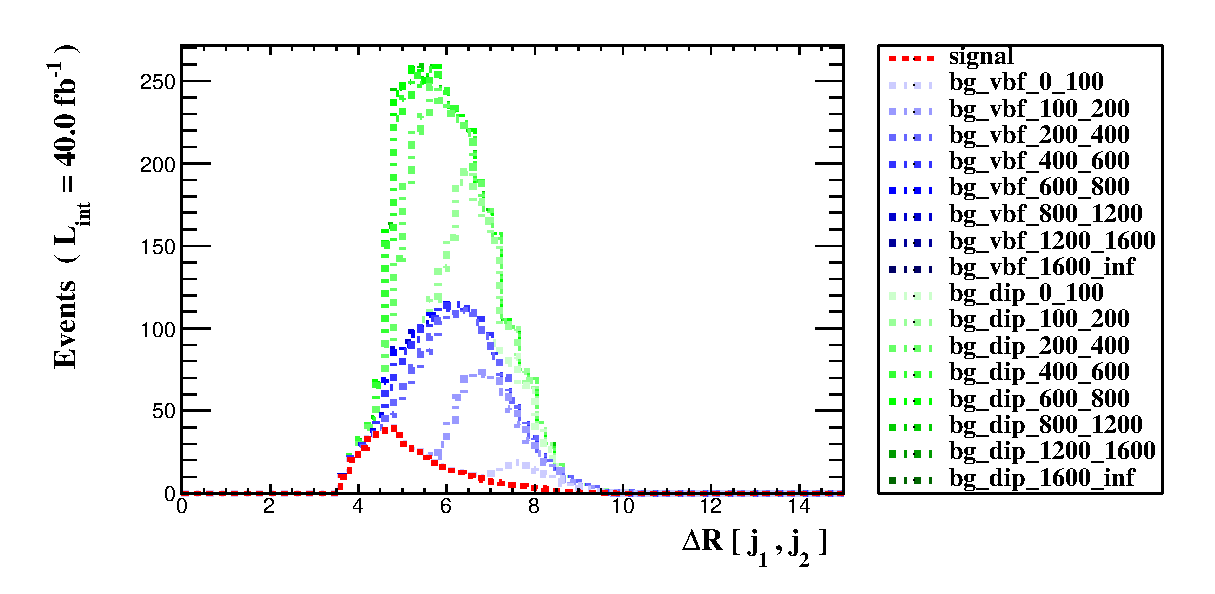
\includegraphics[scale=0.45]{selection_6.eps}\\
\caption{   }
  \end{center}
\end{figure}
      \newpage
\subsection{ Histogram 8}

\textbf{* Plot: M ( jets[1] jets[2] ) }\\
   \begin{table}[H]
  \begin{center}
    \begin{tabular}{|m{23.0mm}|m{23.0mm}|m{18.0mm}|m{19.0mm}|m{19.0mm}|m{19.0mm}|m{19.0mm}|}
      \hline
      {\cellcolor{yellow}         Dataset}& {\cellcolor{yellow}         Integral}& {\cellcolor{yellow}         Entries per event}& {\cellcolor{yellow}         Mean}& {\cellcolor{yellow}         RMS}& {\cellcolor{yellow}         \% underflow}& {\cellcolor{yellow}         \% overflow}\\
      \hline
      {\cellcolor{white}         signal}& {\cellcolor{white}         405}& {\cellcolor{white}         1.0}& {\cellcolor{white}         2092.76}& {\cellcolor{white}         733.8}& {\cellcolor{green}         0.0}& {\cellcolor{green}         0.0}\\
      \hline
      {\cellcolor{white}         bg\_vbf\_0\_100}& {\cellcolor{white}         102}& {\cellcolor{white}         1.0}& {\cellcolor{white}         1754.92}& {\cellcolor{white}         545.8}& {\cellcolor{green}         0.0}& {\cellcolor{green}         0.0}\\
      \hline
      {\cellcolor{white}         bg\_vbf\_100\_200}& {\cellcolor{white}         477}& {\cellcolor{white}         1.0}& {\cellcolor{white}         1797.03}& {\cellcolor{white}         586.5}& {\cellcolor{green}         0.0}& {\cellcolor{green}         0.0}\\
      \hline
      {\cellcolor{white}         bg\_vbf\_200\_400}& {\cellcolor{white}         573}& {\cellcolor{white}         1.0}& {\cellcolor{white}         1935.01}& {\cellcolor{white}         656.1}& {\cellcolor{green}         0.0}& {\cellcolor{green}         0.0}\\
      \hline
      {\cellcolor{white}         bg\_vbf\_400\_600}& {\cellcolor{white}         136}& {\cellcolor{white}         1.0}& {\cellcolor{white}         2182.58}& {\cellcolor{white}         739.7}& {\cellcolor{green}         0.0}& {\cellcolor{green}         0.001443}\\
      \hline
      {\cellcolor{white}         bg\_vbf\_600\_800}& {\cellcolor{white}         23.8}& {\cellcolor{white}         1.0}& {\cellcolor{white}         2781.69}& {\cellcolor{white}         757.5}& {\cellcolor{green}         0.0}& {\cellcolor{green}         0.007403}\\
      \hline
      {\cellcolor{white}         bg\_vbf\_800\_1200}& {\cellcolor{white}         6.04}& {\cellcolor{white}         1.0}& {\cellcolor{white}         3450.11}& {\cellcolor{white}         796.3}& {\cellcolor{green}         0.0}& {\cellcolor{green}         0.02375}\\
      \hline
      {\cellcolor{white}         bg\_vbf\_1200\_1600}& {\cellcolor{white}         0.337}& {\cellcolor{white}         1.0}& {\cellcolor{white}         4535.16}& {\cellcolor{white}         874.5}& {\cellcolor{green}         0.0}& {\cellcolor{green}         0.1026}\\
      \hline
      {\cellcolor{white}         bg\_vbf\_1600\_inf}& {\cellcolor{white}         0.0252}& {\cellcolor{white}         1.0}& {\cellcolor{white}         5588.19}& {\cellcolor{white}         1179}& {\cellcolor{green}         0.0}& {\cellcolor{green}         1.462}\\
      \hline
      {\cellcolor{white}         bg\_dip\_0\_100}& {\cellcolor{white}         117}& {\cellcolor{white}         1.0}& {\cellcolor{white}         1536.49}& {\cellcolor{white}         260.9}& {\cellcolor{green}         0.0}& {\cellcolor{green}         0.0}\\
      \hline
      {\cellcolor{white}         bg\_dip\_100\_200}& {\cellcolor{white}         496}& {\cellcolor{white}         1.0}& {\cellcolor{white}         1527.46}& {\cellcolor{white}         316.0}& {\cellcolor{green}         0.0}& {\cellcolor{green}         0.0}\\
      \hline
      {\cellcolor{white}         bg\_dip\_200\_400}& {\cellcolor{white}         814}& {\cellcolor{white}         1.0}& {\cellcolor{white}         1563.67}& {\cellcolor{white}         323.6}& {\cellcolor{green}         0.0}& {\cellcolor{green}         0.0}\\
      \hline
      {\cellcolor{white}         bg\_dip\_400\_600}& {\cellcolor{white}         292}& {\cellcolor{white}         1.0}& {\cellcolor{white}         1792.15}& {\cellcolor{white}         421.1}& {\cellcolor{green}         0.0}& {\cellcolor{green}         0.0}\\
      \hline
      {\cellcolor{white}         bg\_dip\_600\_800}& {\cellcolor{white}         44.6}& {\cellcolor{white}         1.0}& {\cellcolor{white}         2435.56}& {\cellcolor{white}         527.9}& {\cellcolor{green}         0.0}& {\cellcolor{green}         0.0}\\
      \hline
      {\cellcolor{white}         bg\_dip\_800\_1200}& {\cellcolor{white}         10.9}& {\cellcolor{white}         1.0}& {\cellcolor{white}         3104.76}& {\cellcolor{white}         731.5}& {\cellcolor{green}         0.0}& {\cellcolor{green}         0.0}\\
      \hline
      {\cellcolor{white}         bg\_dip\_1200\_1600}& {\cellcolor{white}         0.675}& {\cellcolor{white}         1.0}& {\cellcolor{white}         4189.44}& {\cellcolor{white}         984.4}& {\cellcolor{green}         0.0}& {\cellcolor{green}         0.0}\\
      \hline
      {\cellcolor{white}         bg\_dip\_1600\_inf}& {\cellcolor{white}         0.0437}& {\cellcolor{white}         1.0}& {\cellcolor{white}         5239.8}& {\cellcolor{white}         1493}& {\cellcolor{green}         0.0}& {\cellcolor{green}         0.414}\\
\hline
    \end{tabular}
  \end{center}
\end{table}

\begin{figure}[H]
  \begin{center}
    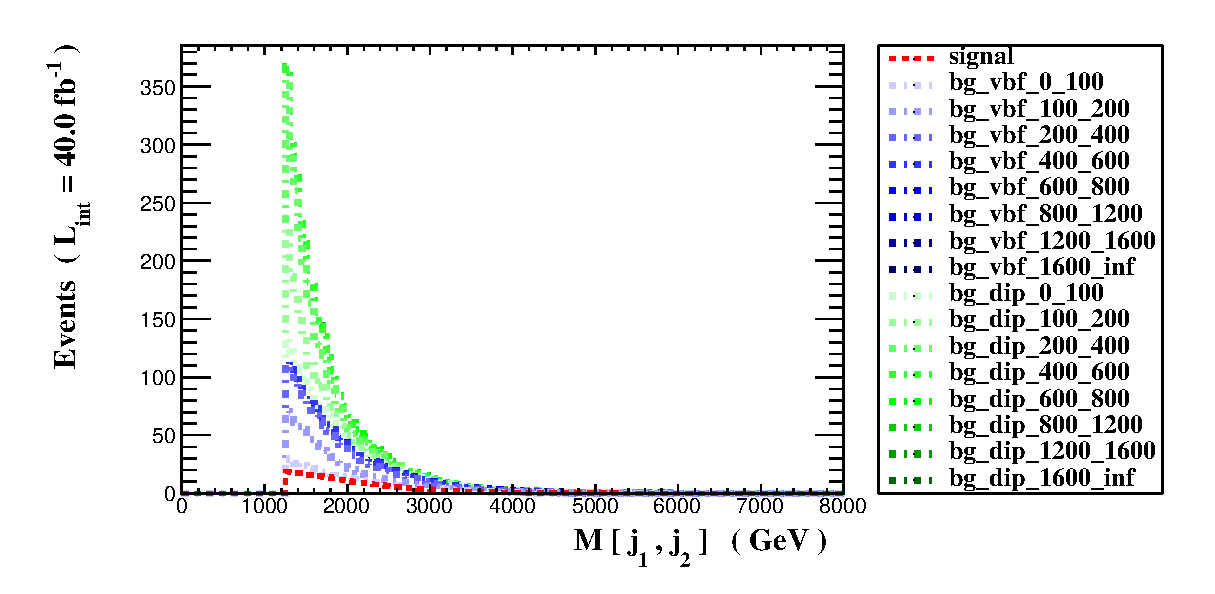
\includegraphics[scale=0.45]{selection_7.eps}\\
\caption{   }
  \end{center}
\end{figure}
      \newpage
\subsection{ Histogram 9}

\textbf{* Plot: MET}\\
   \begin{table}[H]
  \begin{center}
    \begin{tabular}{|m{23.0mm}|m{23.0mm}|m{18.0mm}|m{19.0mm}|m{19.0mm}|m{19.0mm}|m{19.0mm}|}
      \hline
      {\cellcolor{yellow}         Dataset}& {\cellcolor{yellow}         Integral}& {\cellcolor{yellow}         Entries per event}& {\cellcolor{yellow}         Mean}& {\cellcolor{yellow}         RMS}& {\cellcolor{yellow}         \% underflow}& {\cellcolor{yellow}         \% overflow}\\
      \hline
      {\cellcolor{white}         signal}& {\cellcolor{white}         405}& {\cellcolor{white}         1.0}& {\cellcolor{white}         8.08519e-09}& {\cellcolor{white}         1.046e-08}& {\cellcolor{green}         0.0}& {\cellcolor{green}         0.0}\\
      \hline
      {\cellcolor{white}         bg\_vbf\_0\_100}& {\cellcolor{white}         102}& {\cellcolor{white}         1.0}& {\cellcolor{white}         6.19944e-10}& {\cellcolor{white}         4.643e-10}& {\cellcolor{green}         0.0}& {\cellcolor{green}         0.0}\\
      \hline
      {\cellcolor{white}         bg\_vbf\_100\_200}& {\cellcolor{white}         477}& {\cellcolor{white}         1.0}& {\cellcolor{white}         1.03193e-09}& {\cellcolor{white}         1.184e-09}& {\cellcolor{green}         0.0}& {\cellcolor{green}         0.0}\\
      \hline
      {\cellcolor{white}         bg\_vbf\_200\_400}& {\cellcolor{white}         573}& {\cellcolor{white}         1.0}& {\cellcolor{white}         3.36658e-09}& {\cellcolor{white}         2.26e-09}& {\cellcolor{green}         0.0}& {\cellcolor{green}         0.0}\\
      \hline
      {\cellcolor{white}         bg\_vbf\_400\_600}& {\cellcolor{white}         136}& {\cellcolor{white}         1.0}& {\cellcolor{white}         4.57136e-09}& {\cellcolor{white}         2.627e-09}& {\cellcolor{green}         0.0}& {\cellcolor{green}         0.0}\\
      \hline
      {\cellcolor{white}         bg\_vbf\_600\_800}& {\cellcolor{white}         23.8}& {\cellcolor{white}         1.0}& {\cellcolor{white}         4.96532e-09}& {\cellcolor{white}         2.759e-09}& {\cellcolor{green}         0.0}& {\cellcolor{green}         0.0}\\
      \hline
      {\cellcolor{white}         bg\_vbf\_800\_1200}& {\cellcolor{white}         6.04}& {\cellcolor{white}         1.0}& {\cellcolor{white}         5.29507e-09}& {\cellcolor{white}         3.266e-09}& {\cellcolor{green}         0.0}& {\cellcolor{green}         0.0}\\
      \hline
      {\cellcolor{white}         bg\_vbf\_1200\_1600}& {\cellcolor{white}         0.337}& {\cellcolor{white}         1.0}& {\cellcolor{white}         7.57578e-09}& {\cellcolor{white}         9.664e-09}& {\cellcolor{green}         0.0}& {\cellcolor{green}         0.0}\\
      \hline
      {\cellcolor{white}         bg\_vbf\_1600\_inf}& {\cellcolor{white}         0.0252}& {\cellcolor{white}         1.0}& {\cellcolor{white}         1.17343e-08}& {\cellcolor{white}         1.543e-08}& {\cellcolor{green}         0.0}& {\cellcolor{green}         0.0}\\
      \hline
      {\cellcolor{white}         bg\_dip\_0\_100}& {\cellcolor{white}         117}& {\cellcolor{white}         1.0}& {\cellcolor{white}         7.65424e-10}& {\cellcolor{white}         5.853e-10}& {\cellcolor{green}         0.0}& {\cellcolor{green}         0.0}\\
      \hline
      {\cellcolor{white}         bg\_dip\_100\_200}& {\cellcolor{white}         496}& {\cellcolor{white}         1.0}& {\cellcolor{white}         1.18704e-09}& {\cellcolor{white}         1.387e-09}& {\cellcolor{green}         0.0}& {\cellcolor{green}         0.0}\\
      \hline
      {\cellcolor{white}         bg\_dip\_200\_400}& {\cellcolor{white}         814}& {\cellcolor{white}         1.0}& {\cellcolor{white}         3.50088e-09}& {\cellcolor{white}         2.275e-09}& {\cellcolor{green}         0.0}& {\cellcolor{green}         0.0}\\
      \hline
      {\cellcolor{white}         bg\_dip\_400\_600}& {\cellcolor{white}         292}& {\cellcolor{white}         1.0}& {\cellcolor{white}         4.46119e-09}& {\cellcolor{white}         2.584e-09}& {\cellcolor{green}         0.0}& {\cellcolor{green}         0.0}\\
      \hline
      {\cellcolor{white}         bg\_dip\_600\_800}& {\cellcolor{white}         44.6}& {\cellcolor{white}         1.0}& {\cellcolor{white}         4.86013e-09}& {\cellcolor{white}         2.677e-09}& {\cellcolor{green}         0.0}& {\cellcolor{green}         0.0}\\
      \hline
      {\cellcolor{white}         bg\_dip\_800\_1200}& {\cellcolor{white}         10.9}& {\cellcolor{white}         1.0}& {\cellcolor{white}         5.19487e-09}& {\cellcolor{white}         4.117e-09}& {\cellcolor{green}         0.0}& {\cellcolor{green}         0.0}\\
      \hline
      {\cellcolor{white}         bg\_dip\_1200\_1600}& {\cellcolor{white}         0.675}& {\cellcolor{white}         1.0}& {\cellcolor{white}         8.45939e-09}& {\cellcolor{white}         1.179e-08}& {\cellcolor{green}         0.0}& {\cellcolor{green}         0.0}\\
      \hline
      {\cellcolor{white}         bg\_dip\_1600\_inf}& {\cellcolor{white}         0.0437}& {\cellcolor{white}         1.0}& {\cellcolor{white}         1.08698e-08}& {\cellcolor{white}         1.476e-08}& {\cellcolor{green}         0.0}& {\cellcolor{green}         0.0}\\
\hline
    \end{tabular}
  \end{center}
\end{table}

\begin{figure}[H]
  \begin{center}
    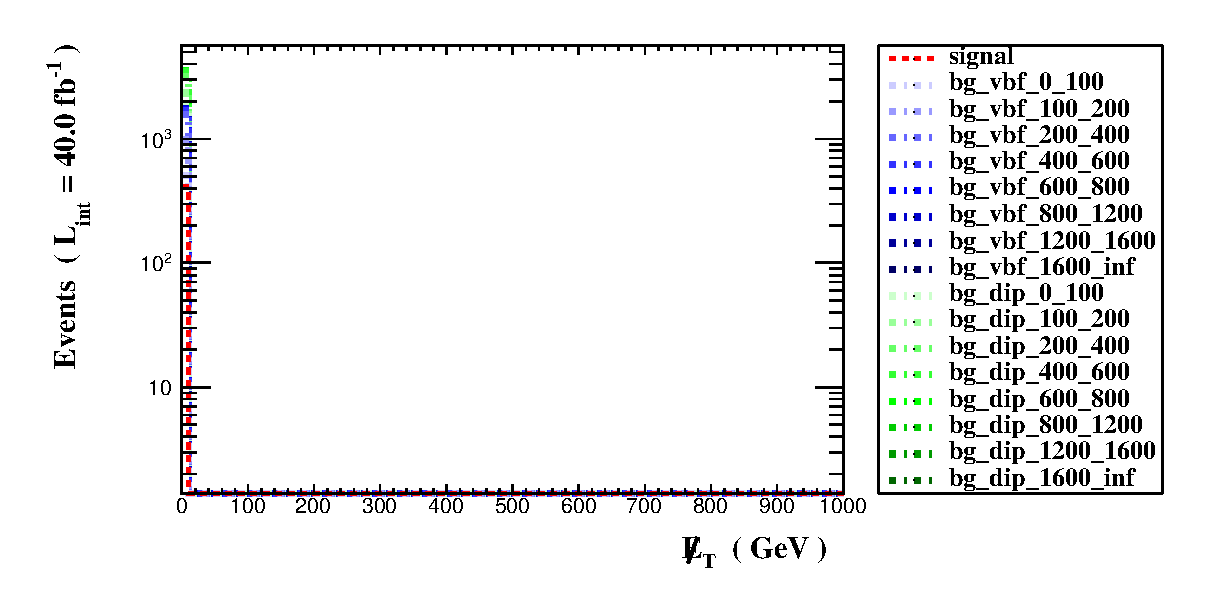
\includegraphics[scale=0.45]{selection_8.eps}\\
\caption{   }
  \end{center}
\end{figure}
      \newpage
\subsection{ Histogram 10}

\textbf{* Plot: sdETA ( jets[1] jets[2] ) }\\
   \begin{table}[H]
  \begin{center}
    \begin{tabular}{|m{23.0mm}|m{23.0mm}|m{18.0mm}|m{19.0mm}|m{19.0mm}|m{19.0mm}|m{19.0mm}|}
      \hline
      {\cellcolor{yellow}         Dataset}& {\cellcolor{yellow}         Integral}& {\cellcolor{yellow}         Entries per event}& {\cellcolor{yellow}         Mean}& {\cellcolor{yellow}         RMS}& {\cellcolor{yellow}         \% underflow}& {\cellcolor{yellow}         \% overflow}\\
      \hline
      {\cellcolor{white}         signal}& {\cellcolor{white}         405}& {\cellcolor{white}         1.0}& {\cellcolor{white}         4.93861}& {\cellcolor{white}         1.162}& {\cellcolor{green}         0.0}& {\cellcolor{green}         2.039}\\
      \hline
      {\cellcolor{white}         bg\_vbf\_0\_100}& {\cellcolor{white}         102}& {\cellcolor{white}         1.0}& {\cellcolor{white}         7.57435}& {\cellcolor{white}         0.6115}& {\cellcolor{red}         0.0}& {\cellcolor{red}         23.21}\\
      \hline
      {\cellcolor{white}         bg\_vbf\_100\_200}& {\cellcolor{white}         477}& {\cellcolor{white}         1.0}& {\cellcolor{white}         6.40026}& {\cellcolor{white}         0.6673}& {\cellcolor{green}         0.0}& {\cellcolor{green}         2.156}\\
      \hline
      {\cellcolor{white}         bg\_vbf\_200\_400}& {\cellcolor{white}         573}& {\cellcolor{white}         1.0}& {\cellcolor{white}         5.25178}& {\cellcolor{white}         0.7177}& {\cellcolor{green}         0.0}& {\cellcolor{green}         0.03453}\\
      \hline
      {\cellcolor{white}         bg\_vbf\_400\_600}& {\cellcolor{white}         136}& {\cellcolor{white}         1.0}& {\cellcolor{white}         4.41616}& {\cellcolor{white}         0.6066}& {\cellcolor{green}         0.0}& {\cellcolor{green}         0.0}\\
      \hline
      {\cellcolor{white}         bg\_vbf\_600\_800}& {\cellcolor{white}         23.8}& {\cellcolor{white}         1.0}& {\cellcolor{white}         4.22247}& {\cellcolor{white}         0.4867}& {\cellcolor{green}         0.0}& {\cellcolor{green}         0.0}\\
      \hline
      {\cellcolor{white}         bg\_vbf\_800\_1200}& {\cellcolor{white}         6.04}& {\cellcolor{white}         1.0}& {\cellcolor{white}         4.07691}& {\cellcolor{white}         0.392}& {\cellcolor{green}         0.0}& {\cellcolor{green}         0.0}\\
      \hline
      {\cellcolor{white}         bg\_vbf\_1200\_1600}& {\cellcolor{white}         0.337}& {\cellcolor{white}         1.0}& {\cellcolor{white}         3.93047}& {\cellcolor{white}         0.2943}& {\cellcolor{green}         0.0}& {\cellcolor{green}         0.0}\\
      \hline
      {\cellcolor{white}         bg\_vbf\_1600\_inf}& {\cellcolor{white}         0.0252}& {\cellcolor{white}         1.0}& {\cellcolor{white}         3.84737}& {\cellcolor{white}         0.2443}& {\cellcolor{green}         0.0}& {\cellcolor{green}         0.0}\\
      \hline
      {\cellcolor{white}         bg\_dip\_0\_100}& {\cellcolor{white}         117}& {\cellcolor{white}         1.0}& {\cellcolor{white}         7.31275}& {\cellcolor{white}         0.3459}& {\cellcolor{green}         0.0}& {\cellcolor{green}         4.448}\\
      \hline
      {\cellcolor{white}         bg\_dip\_100\_200}& {\cellcolor{white}         496}& {\cellcolor{white}         1.0}& {\cellcolor{white}         6.11125}& {\cellcolor{white}         0.5289}& {\cellcolor{green}         0.0}& {\cellcolor{green}         0.0}\\
      \hline
      {\cellcolor{white}         bg\_dip\_200\_400}& {\cellcolor{white}         814}& {\cellcolor{white}         1.0}& {\cellcolor{white}         4.81866}& {\cellcolor{white}         0.5746}& {\cellcolor{green}         0.0}& {\cellcolor{green}         0.0}\\
      \hline
      {\cellcolor{white}         bg\_dip\_400\_600}& {\cellcolor{white}         292}& {\cellcolor{white}         1.0}& {\cellcolor{white}         4.08668}& {\cellcolor{white}         0.4285}& {\cellcolor{green}         0.0}& {\cellcolor{green}         0.0}\\
      \hline
      {\cellcolor{white}         bg\_dip\_600\_800}& {\cellcolor{white}         44.6}& {\cellcolor{white}         1.0}& {\cellcolor{white}         4.01403}& {\cellcolor{white}         0.3681}& {\cellcolor{green}         0.0}& {\cellcolor{green}         0.0}\\
      \hline
      {\cellcolor{white}         bg\_dip\_800\_1200}& {\cellcolor{white}         10.9}& {\cellcolor{white}         1.0}& {\cellcolor{white}         3.95789}& {\cellcolor{white}         0.3287}& {\cellcolor{green}         0.0}& {\cellcolor{green}         0.0}\\
      \hline
      {\cellcolor{white}         bg\_dip\_1200\_1600}& {\cellcolor{white}         0.675}& {\cellcolor{white}         1.0}& {\cellcolor{white}         3.86566}& {\cellcolor{white}         0.2738}& {\cellcolor{green}         0.0}& {\cellcolor{green}         0.0}\\
      \hline
      {\cellcolor{white}         bg\_dip\_1600\_inf}& {\cellcolor{white}         0.0437}& {\cellcolor{white}         1.0}& {\cellcolor{white}         3.81916}& {\cellcolor{white}         0.2447}& {\cellcolor{green}         0.0}& {\cellcolor{green}         0.0}\\
\hline
    \end{tabular}
  \end{center}
\end{table}

\begin{figure}[H]
  \begin{center}
    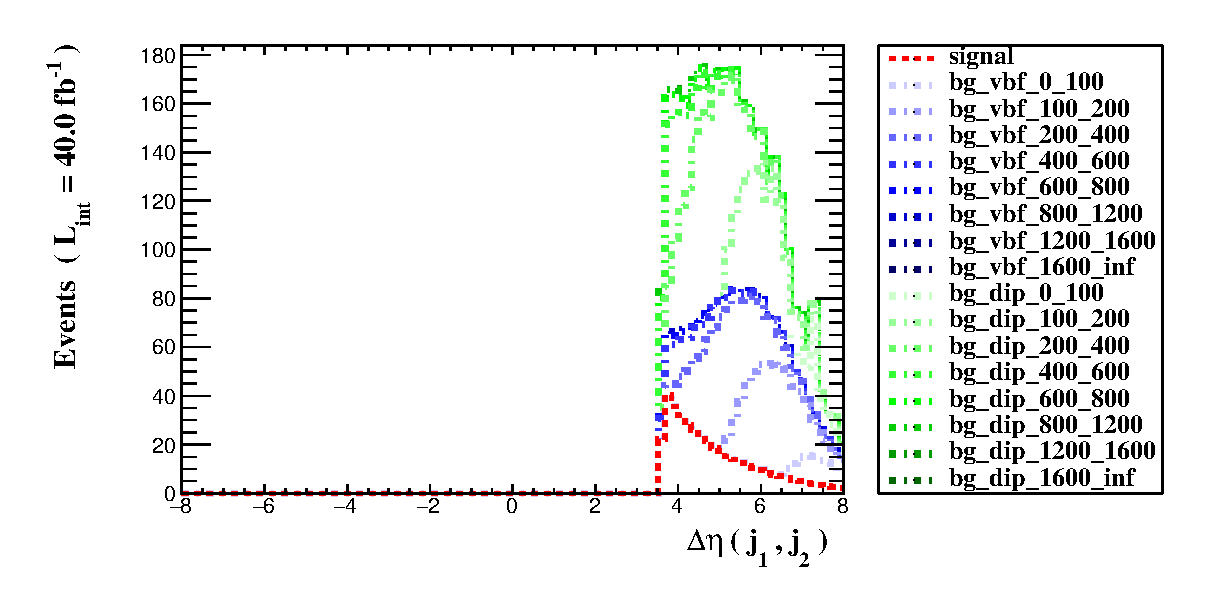
\includegraphics[scale=0.45]{selection_9.eps}\\
\caption{   }
  \end{center}
\end{figure}
      \newpage
\subsection{ Histogram 11}

\textbf{* Plot: M ( a[1] a[2] ) }\\
   \begin{table}[H]
  \begin{center}
    \begin{tabular}{|m{23.0mm}|m{23.0mm}|m{18.0mm}|m{19.0mm}|m{19.0mm}|m{19.0mm}|m{19.0mm}|}
      \hline
      {\cellcolor{yellow}         Dataset}& {\cellcolor{yellow}         Integral}& {\cellcolor{yellow}         Entries per event}& {\cellcolor{yellow}         Mean}& {\cellcolor{yellow}         RMS}& {\cellcolor{yellow}         \% underflow}& {\cellcolor{yellow}         \% overflow}\\
      \hline
      {\cellcolor{white}         signal}& {\cellcolor{white}         405}& {\cellcolor{white}         1.0}& {\cellcolor{white}         1033.19}& {\cellcolor{white}         770.9}& {\cellcolor{red}         0.0}& {\cellcolor{red}         41.25}\\
      \hline
      {\cellcolor{white}         bg\_vbf\_0\_100}& {\cellcolor{white}         102}& {\cellcolor{white}         1.0}& {\cellcolor{white}         74.8671}& {\cellcolor{white}         64.42}& {\cellcolor{green}         0.0}& {\cellcolor{green}         0.01176}\\
      \hline
      {\cellcolor{white}         bg\_vbf\_100\_200}& {\cellcolor{white}         477}& {\cellcolor{white}         1.0}& {\cellcolor{white}         89.3839}& {\cellcolor{white}         83.48}& {\cellcolor{green}         0.0}& {\cellcolor{green}         0.0399}\\
      \hline
      {\cellcolor{white}         bg\_vbf\_200\_400}& {\cellcolor{white}         573}& {\cellcolor{white}         1.0}& {\cellcolor{white}         113.725}& {\cellcolor{white}         113.1}& {\cellcolor{green}         0.0}& {\cellcolor{green}         0.1218}\\
      \hline
      {\cellcolor{white}         bg\_vbf\_400\_600}& {\cellcolor{white}         136}& {\cellcolor{white}         1.0}& {\cellcolor{white}         139.497}& {\cellcolor{white}         143.5}& {\cellcolor{green}         0.0}& {\cellcolor{green}         0.2771}\\
      \hline
      {\cellcolor{white}         bg\_vbf\_600\_800}& {\cellcolor{white}         23.8}& {\cellcolor{white}         1.0}& {\cellcolor{white}         165.376}& {\cellcolor{white}         176.9}& {\cellcolor{green}         0.0}& {\cellcolor{green}         0.6767}\\
      \hline
      {\cellcolor{white}         bg\_vbf\_800\_1200}& {\cellcolor{white}         6.04}& {\cellcolor{white}         1.0}& {\cellcolor{white}         184.367}& {\cellcolor{white}         198.5}& {\cellcolor{green}         0.0}& {\cellcolor{green}         0.9958}\\
      \hline
      {\cellcolor{white}         bg\_vbf\_1200\_1600}& {\cellcolor{white}         0.337}& {\cellcolor{white}         1.0}& {\cellcolor{white}         211.673}& {\cellcolor{white}         240.5}& {\cellcolor{green}         0.0}& {\cellcolor{green}         1.847}\\
      \hline
      {\cellcolor{white}         bg\_vbf\_1600\_inf}& {\cellcolor{white}         0.0252}& {\cellcolor{white}         1.0}& {\cellcolor{white}         258.692}& {\cellcolor{white}         305.6}& {\cellcolor{green}         0.0}& {\cellcolor{green}         3.602}\\
      \hline
      {\cellcolor{white}         bg\_dip\_0\_100}& {\cellcolor{white}         117}& {\cellcolor{white}         1.0}& {\cellcolor{white}         67.9791}& {\cellcolor{white}         48.97}& {\cellcolor{green}         0.0}& {\cellcolor{green}         0.0}\\
      \hline
      {\cellcolor{white}         bg\_dip\_100\_200}& {\cellcolor{white}         496}& {\cellcolor{white}         1.0}& {\cellcolor{white}         81.4606}& {\cellcolor{white}         86.76}& {\cellcolor{green}         0.0}& {\cellcolor{green}         0.0}\\
      \hline
      {\cellcolor{white}         bg\_dip\_200\_400}& {\cellcolor{white}         814}& {\cellcolor{white}         1.0}& {\cellcolor{white}         101.829}& {\cellcolor{white}         117.4}& {\cellcolor{green}         0.0}& {\cellcolor{green}         0.08477}\\
      \hline
      {\cellcolor{white}         bg\_dip\_400\_600}& {\cellcolor{white}         292}& {\cellcolor{white}         1.0}& {\cellcolor{white}         128.284}& {\cellcolor{white}         156.9}& {\cellcolor{green}         0.0}& {\cellcolor{green}         0.4064}\\
      \hline
      {\cellcolor{white}         bg\_dip\_600\_800}& {\cellcolor{white}         44.6}& {\cellcolor{white}         1.0}& {\cellcolor{white}         159.226}& {\cellcolor{white}         192.7}& {\cellcolor{green}         0.0}& {\cellcolor{green}         0.882}\\
      \hline
      {\cellcolor{white}         bg\_dip\_800\_1200}& {\cellcolor{white}         10.9}& {\cellcolor{white}         1.0}& {\cellcolor{white}         192.169}& {\cellcolor{white}         228.1}& {\cellcolor{green}         0.0}& {\cellcolor{green}         1.247}\\
      \hline
      {\cellcolor{white}         bg\_dip\_1200\_1600}& {\cellcolor{white}         0.675}& {\cellcolor{white}         1.0}& {\cellcolor{white}         219.108}& {\cellcolor{white}         274.9}& {\cellcolor{green}         0.0}& {\cellcolor{green}         2.71}\\
      \hline
      {\cellcolor{white}         bg\_dip\_1600\_inf}& {\cellcolor{white}         0.0437}& {\cellcolor{white}         1.0}& {\cellcolor{white}         276.432}& {\cellcolor{white}         301.7}& {\cellcolor{green}         0.0}& {\cellcolor{green}         2.477}\\
\hline
    \end{tabular}
  \end{center}
\end{table}

\begin{figure}[H]
  \begin{center}
    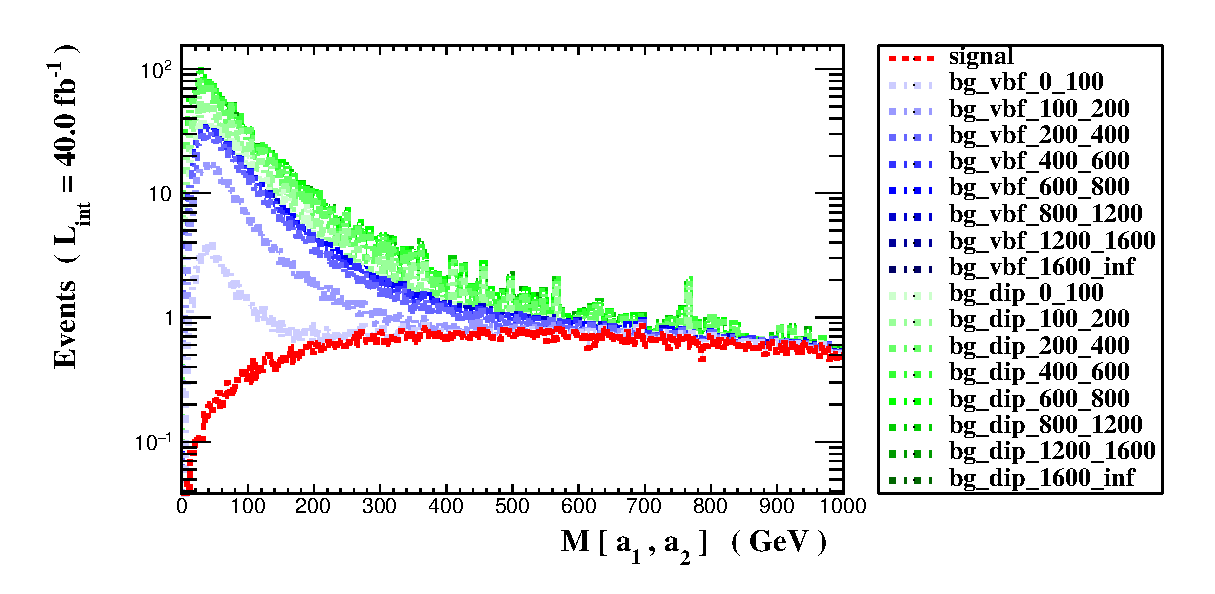
\includegraphics[scale=0.45]{selection_10.eps}\\
\caption{   }
  \end{center}
\end{figure}
      \newpage
\subsection{ Histogram 12}

\textbf{* Plot: PT ( a[1] ) }\\
   \begin{table}[H]
  \begin{center}
    \begin{tabular}{|m{23.0mm}|m{23.0mm}|m{18.0mm}|m{19.0mm}|m{19.0mm}|m{19.0mm}|m{19.0mm}|}
      \hline
      {\cellcolor{yellow}         Dataset}& {\cellcolor{yellow}         Integral}& {\cellcolor{yellow}         Entries per event}& {\cellcolor{yellow}         Mean}& {\cellcolor{yellow}         RMS}& {\cellcolor{yellow}         \% underflow}& {\cellcolor{yellow}         \% overflow}\\
      \hline
      {\cellcolor{white}         signal}& {\cellcolor{white}         405}& {\cellcolor{white}         1.0}& {\cellcolor{white}         592.21}& {\cellcolor{white}         364.8}& {\cellcolor{orange}         0.0}& {\cellcolor{orange}         12.6}\\
      \hline
      {\cellcolor{white}         bg\_vbf\_0\_100}& {\cellcolor{white}         102}& {\cellcolor{white}         1.0}& {\cellcolor{white}         37.6561}& {\cellcolor{white}         21.46}& {\cellcolor{green}         0.0}& {\cellcolor{green}         0.0}\\
      \hline
      {\cellcolor{white}         bg\_vbf\_100\_200}& {\cellcolor{white}         477}& {\cellcolor{white}         1.0}& {\cellcolor{white}         51.7205}& {\cellcolor{white}         34.53}& {\cellcolor{green}         0.0}& {\cellcolor{green}         0.0}\\
      \hline
      {\cellcolor{white}         bg\_vbf\_200\_400}& {\cellcolor{white}         573}& {\cellcolor{white}         1.0}& {\cellcolor{white}         79.4071}& {\cellcolor{white}         64.6}& {\cellcolor{green}         0.0}& {\cellcolor{green}         0.0}\\
      \hline
      {\cellcolor{white}         bg\_vbf\_400\_600}& {\cellcolor{white}         136}& {\cellcolor{white}         1.0}& {\cellcolor{white}         120.13}& {\cellcolor{white}         110.2}& {\cellcolor{green}         0.0}& {\cellcolor{green}         0.002886}\\
      \hline
      {\cellcolor{white}         bg\_vbf\_600\_800}& {\cellcolor{white}         23.8}& {\cellcolor{white}         1.0}& {\cellcolor{white}         162.739}& {\cellcolor{white}         163.7}& {\cellcolor{green}         0.0}& {\cellcolor{green}         0.0148}\\
      \hline
      {\cellcolor{white}         bg\_vbf\_800\_1200}& {\cellcolor{white}         6.04}& {\cellcolor{white}         1.0}& {\cellcolor{white}         205.495}& {\cellcolor{white}         231.0}& {\cellcolor{green}         0.0}& {\cellcolor{green}         0.7822}\\
      \hline
      {\cellcolor{white}         bg\_vbf\_1200\_1600}& {\cellcolor{white}         0.337}& {\cellcolor{white}         1.0}& {\cellcolor{white}         277.542}& {\cellcolor{white}         353.0}& {\cellcolor{orange}         0.0}& {\cellcolor{orange}         8.228}\\
      \hline
      {\cellcolor{white}         bg\_vbf\_1600\_inf}& {\cellcolor{white}         0.0252}& {\cellcolor{white}         1.0}& {\cellcolor{white}         395.601}& {\cellcolor{white}         548.9}& {\cellcolor{red}         0.0}& {\cellcolor{red}         15.97}\\
      \hline
      {\cellcolor{white}         bg\_dip\_0\_100}& {\cellcolor{white}         117}& {\cellcolor{white}         1.0}& {\cellcolor{white}         39.6474}& {\cellcolor{white}         25.66}& {\cellcolor{green}         0.0}& {\cellcolor{green}         0.0}\\
      \hline
      {\cellcolor{white}         bg\_dip\_100\_200}& {\cellcolor{white}         496}& {\cellcolor{white}         1.0}& {\cellcolor{white}         55.7039}& {\cellcolor{white}         43.6}& {\cellcolor{green}         0.0}& {\cellcolor{green}         0.0}\\
      \hline
      {\cellcolor{white}         bg\_dip\_200\_400}& {\cellcolor{white}         814}& {\cellcolor{white}         1.0}& {\cellcolor{white}         77.1175}& {\cellcolor{white}         73.41}& {\cellcolor{green}         0.0}& {\cellcolor{green}         0.0}\\
      \hline
      {\cellcolor{white}         bg\_dip\_400\_600}& {\cellcolor{white}         292}& {\cellcolor{white}         1.0}& {\cellcolor{white}         101.734}& {\cellcolor{white}         112.2}& {\cellcolor{green}         0.0}& {\cellcolor{green}         0.0}\\
      \hline
      {\cellcolor{white}         bg\_dip\_600\_800}& {\cellcolor{white}         44.6}& {\cellcolor{white}         1.0}& {\cellcolor{white}         143.507}& {\cellcolor{white}         174.0}& {\cellcolor{green}         0.0}& {\cellcolor{green}         0.02262}\\
      \hline
      {\cellcolor{white}         bg\_dip\_800\_1200}& {\cellcolor{white}         10.9}& {\cellcolor{white}         1.0}& {\cellcolor{white}         205.072}& {\cellcolor{white}         276.7}& {\cellcolor{green}         0.0}& {\cellcolor{green}         1.974}\\
      \hline
      {\cellcolor{white}         bg\_dip\_1200\_1600}& {\cellcolor{white}         0.675}& {\cellcolor{white}         1.0}& {\cellcolor{white}         274.485}& {\cellcolor{white}         426.3}& {\cellcolor{orange}         0.0}& {\cellcolor{orange}         13.32}\\
      \hline
      {\cellcolor{white}         bg\_dip\_1600\_inf}& {\cellcolor{white}         0.0437}& {\cellcolor{white}         1.0}& {\cellcolor{white}         399.282}& {\cellcolor{white}         651.2}& {\cellcolor{red}         0.0}& {\cellcolor{red}         17.36}\\
\hline
    \end{tabular}
  \end{center}
\end{table}

\begin{figure}[H]
  \begin{center}
    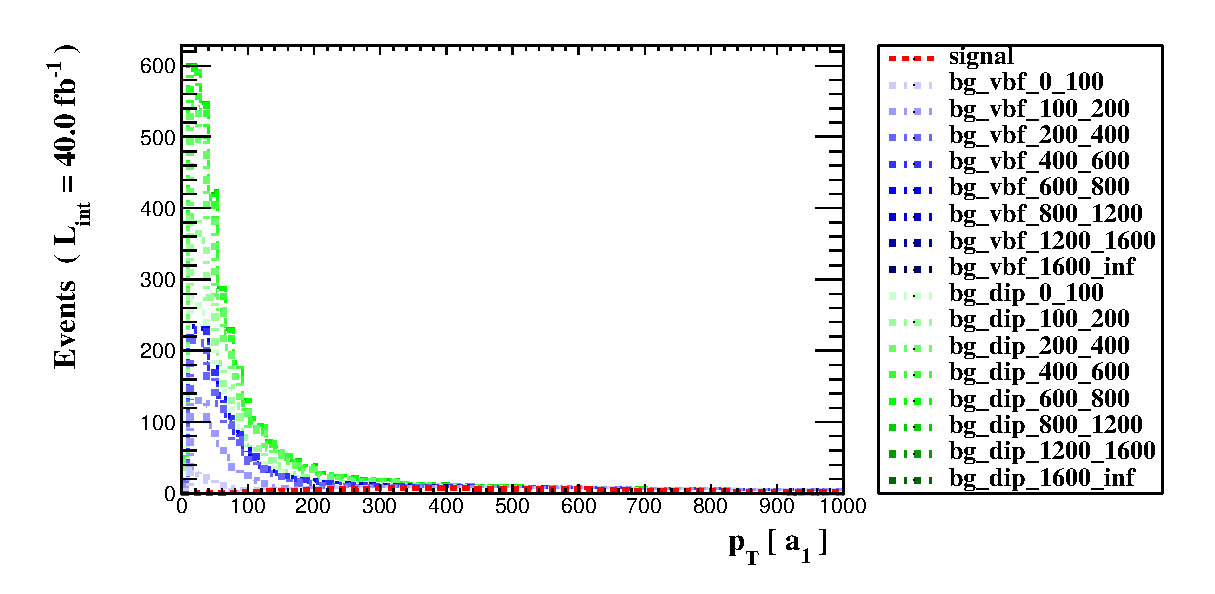
\includegraphics[scale=0.45]{selection_11.eps}\\
\caption{   }
  \end{center}
\end{figure}
      \newpage
\subsection{ Histogram 13}

\textbf{* Plot: PT ( a[2] ) }\\
   \begin{table}[H]
  \begin{center}
    \begin{tabular}{|m{23.0mm}|m{23.0mm}|m{18.0mm}|m{19.0mm}|m{19.0mm}|m{19.0mm}|m{19.0mm}|}
      \hline
      {\cellcolor{yellow}         Dataset}& {\cellcolor{yellow}         Integral}& {\cellcolor{yellow}         Entries per event}& {\cellcolor{yellow}         Mean}& {\cellcolor{yellow}         RMS}& {\cellcolor{yellow}         \% underflow}& {\cellcolor{yellow}         \% overflow}\\
      \hline
      {\cellcolor{white}         signal}& {\cellcolor{white}         405}& {\cellcolor{white}         1.0}& {\cellcolor{white}         362.444}& {\cellcolor{white}         311.6}& {\cellcolor{green}         0.0}& {\cellcolor{green}         4.721}\\
      \hline
      {\cellcolor{white}         bg\_vbf\_0\_100}& {\cellcolor{white}         102}& {\cellcolor{white}         1.0}& {\cellcolor{white}         19.9879}& {\cellcolor{white}         13.16}& {\cellcolor{green}         0.0}& {\cellcolor{green}         0.0}\\
      \hline
      {\cellcolor{white}         bg\_vbf\_100\_200}& {\cellcolor{white}         477}& {\cellcolor{white}         1.0}& {\cellcolor{white}         23.3502}& {\cellcolor{white}         18.44}& {\cellcolor{green}         0.0}& {\cellcolor{green}         0.0}\\
      \hline
      {\cellcolor{white}         bg\_vbf\_200\_400}& {\cellcolor{white}         573}& {\cellcolor{white}         1.0}& {\cellcolor{white}         28.1052}& {\cellcolor{white}         26.02}& {\cellcolor{green}         0.0}& {\cellcolor{green}         0.0}\\
      \hline
      {\cellcolor{white}         bg\_vbf\_400\_600}& {\cellcolor{white}         136}& {\cellcolor{white}         1.0}& {\cellcolor{white}         33.8376}& {\cellcolor{white}         35.49}& {\cellcolor{green}         0.0}& {\cellcolor{green}         0.0}\\
      \hline
      {\cellcolor{white}         bg\_vbf\_600\_800}& {\cellcolor{white}         23.8}& {\cellcolor{white}         1.0}& {\cellcolor{white}         38.9053}& {\cellcolor{white}         45.07}& {\cellcolor{green}         0.0}& {\cellcolor{green}         0.001058}\\
      \hline
      {\cellcolor{white}         bg\_vbf\_800\_1200}& {\cellcolor{white}         6.04}& {\cellcolor{white}         1.0}& {\cellcolor{white}         42.0948}& {\cellcolor{white}         52.87}& {\cellcolor{green}         0.0}& {\cellcolor{green}         0.0}\\
      \hline
      {\cellcolor{white}         bg\_vbf\_1200\_1600}& {\cellcolor{white}         0.337}& {\cellcolor{white}         1.0}& {\cellcolor{white}         47.3593}& {\cellcolor{white}         66.98}& {\cellcolor{green}         0.0}& {\cellcolor{green}         0.01921}\\
      \hline
      {\cellcolor{white}         bg\_vbf\_1600\_inf}& {\cellcolor{white}         0.0252}& {\cellcolor{white}         1.0}& {\cellcolor{white}         56.8733}& {\cellcolor{white}         90.0}& {\cellcolor{green}         0.0}& {\cellcolor{green}         0.1126}\\
      \hline
      {\cellcolor{white}         bg\_dip\_0\_100}& {\cellcolor{white}         117}& {\cellcolor{white}         1.0}& {\cellcolor{white}         21.3156}& {\cellcolor{white}         12.28}& {\cellcolor{green}         0.0}& {\cellcolor{green}         0.0}\\
      \hline
      {\cellcolor{white}         bg\_dip\_100\_200}& {\cellcolor{white}         496}& {\cellcolor{white}         1.0}& {\cellcolor{white}         21.5768}& {\cellcolor{white}         16.61}& {\cellcolor{green}         0.0}& {\cellcolor{green}         0.0}\\
      \hline
      {\cellcolor{white}         bg\_dip\_200\_400}& {\cellcolor{white}         814}& {\cellcolor{white}         1.0}& {\cellcolor{white}         24.8054}& {\cellcolor{white}         22.89}& {\cellcolor{green}         0.0}& {\cellcolor{green}         0.0}\\
      \hline
      {\cellcolor{white}         bg\_dip\_400\_600}& {\cellcolor{white}         292}& {\cellcolor{white}         1.0}& {\cellcolor{white}         27.9732}& {\cellcolor{white}         28.27}& {\cellcolor{green}         0.0}& {\cellcolor{green}         0.0}\\
      \hline
      {\cellcolor{white}         bg\_dip\_600\_800}& {\cellcolor{white}         44.6}& {\cellcolor{white}         1.0}& {\cellcolor{white}         31.8662}& {\cellcolor{white}         36.74}& {\cellcolor{green}         0.0}& {\cellcolor{green}         0.0}\\
      \hline
      {\cellcolor{white}         bg\_dip\_800\_1200}& {\cellcolor{white}         10.9}& {\cellcolor{white}         1.0}& {\cellcolor{white}         34.9499}& {\cellcolor{white}         43.35}& {\cellcolor{green}         0.0}& {\cellcolor{green}         0.0}\\
      \hline
      {\cellcolor{white}         bg\_dip\_1200\_1600}& {\cellcolor{white}         0.675}& {\cellcolor{white}         1.0}& {\cellcolor{white}         41.3463}& {\cellcolor{white}         66.97}& {\cellcolor{green}         0.0}& {\cellcolor{green}         0.0}\\
      \hline
      {\cellcolor{white}         bg\_dip\_1600\_inf}& {\cellcolor{white}         0.0437}& {\cellcolor{white}         1.0}& {\cellcolor{white}         37.3756}& {\cellcolor{white}         50.21}& {\cellcolor{green}         0.0}& {\cellcolor{green}         0.0}\\
\hline
    \end{tabular}
  \end{center}
\end{table}

\begin{figure}[H]
  \begin{center}
    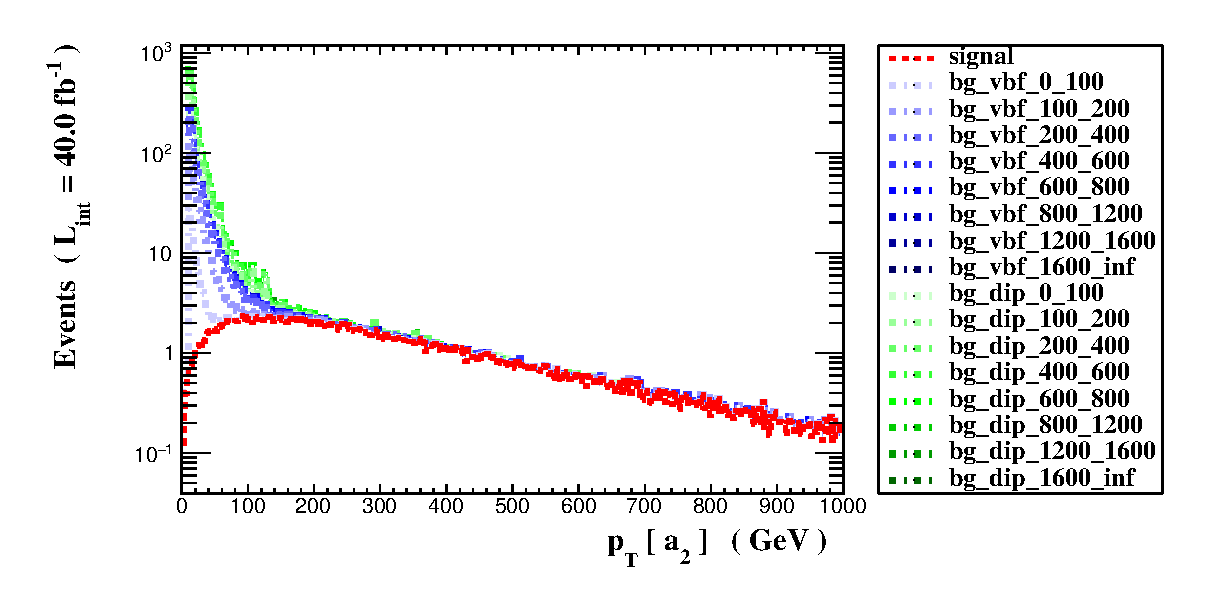
\includegraphics[scale=0.45]{selection_12.eps}\\
\caption{   }
  \end{center}
\end{figure}
      \newpage
\subsection{ Histogram 14}

\textbf{* Plot: THT}\\
   \begin{table}[H]
  \begin{center}
    \begin{tabular}{|m{23.0mm}|m{23.0mm}|m{18.0mm}|m{19.0mm}|m{19.0mm}|m{19.0mm}|m{19.0mm}|}
      \hline
      {\cellcolor{yellow}         Dataset}& {\cellcolor{yellow}         Integral}& {\cellcolor{yellow}         Entries per event}& {\cellcolor{yellow}         Mean}& {\cellcolor{yellow}         RMS}& {\cellcolor{yellow}         \% underflow}& {\cellcolor{yellow}         \% overflow}\\
      \hline
      {\cellcolor{white}         signal}& {\cellcolor{white}         405}& {\cellcolor{white}         1.0}& {\cellcolor{white}         507.51}& {\cellcolor{white}         301.7}& {\cellcolor{orange}         0.0}& {\cellcolor{orange}         6.672}\\
      \hline
      {\cellcolor{white}         bg\_vbf\_0\_100}& {\cellcolor{white}         102}& {\cellcolor{white}         1.0}& {\cellcolor{white}         80.0995}& {\cellcolor{white}         13.51}& {\cellcolor{green}         0.0}& {\cellcolor{green}         0.0}\\
      \hline
      {\cellcolor{white}         bg\_vbf\_100\_200}& {\cellcolor{white}         477}& {\cellcolor{white}         1.0}& {\cellcolor{white}         148.512}& {\cellcolor{white}         28.32}& {\cellcolor{green}         0.0}& {\cellcolor{green}         0.0}\\
      \hline
      {\cellcolor{white}         bg\_vbf\_200\_400}& {\cellcolor{white}         573}& {\cellcolor{white}         1.0}& {\cellcolor{white}         280.111}& {\cellcolor{white}         55.42}& {\cellcolor{green}         0.0}& {\cellcolor{green}         0.0}\\
      \hline
      {\cellcolor{white}         bg\_vbf\_400\_600}& {\cellcolor{white}         136}& {\cellcolor{white}         1.0}& {\cellcolor{white}         470.879}& {\cellcolor{white}         53.35}& {\cellcolor{green}         0.0}& {\cellcolor{green}         0.0}\\
      \hline
      {\cellcolor{white}         bg\_vbf\_600\_800}& {\cellcolor{white}         23.8}& {\cellcolor{white}         1.0}& {\cellcolor{white}         673.777}& {\cellcolor{white}         54.21}& {\cellcolor{green}         0.0}& {\cellcolor{green}         0.0}\\
      \hline
      {\cellcolor{white}         bg\_vbf\_800\_1200}& {\cellcolor{white}         6.04}& {\cellcolor{white}         1.0}& {\cellcolor{white}         913.6}& {\cellcolor{white}         95.92}& {\cellcolor{red}         0.0}& {\cellcolor{red}         19.0}\\
      \hline
      {\cellcolor{white}         bg\_vbf\_1200\_1600}& {\cellcolor{white}         0.337}& {\cellcolor{white}         1.0}& {\cellcolor{white}         1316.92}& {\cellcolor{white}         95.9}& {\cellcolor{red}         0.0}& {\cellcolor{red}         100.0}\\
      \hline
      {\cellcolor{white}         bg\_vbf\_1600\_inf}& {\cellcolor{white}         0.0252}& {\cellcolor{white}         1.0}& {\cellcolor{white}         1746.1}& {\cellcolor{white}         152.6}& {\cellcolor{red}         0.0}& {\cellcolor{red}         100.0}\\
      \hline
      {\cellcolor{white}         bg\_dip\_0\_100}& {\cellcolor{white}         117}& {\cellcolor{white}         1.0}& {\cellcolor{white}         81.8197}& {\cellcolor{white}         10.1}& {\cellcolor{green}         0.0}& {\cellcolor{green}         0.0}\\
      \hline
      {\cellcolor{white}         bg\_dip\_100\_200}& {\cellcolor{white}         496}& {\cellcolor{white}         1.0}& {\cellcolor{white}         150.725}& {\cellcolor{white}         28.95}& {\cellcolor{green}         0.0}& {\cellcolor{green}         0.0}\\
      \hline
      {\cellcolor{white}         bg\_dip\_200\_400}& {\cellcolor{white}         814}& {\cellcolor{white}         1.0}& {\cellcolor{white}         291.464}& {\cellcolor{white}         57.47}& {\cellcolor{green}         0.0}& {\cellcolor{green}         0.0}\\
      \hline
      {\cellcolor{white}         bg\_dip\_400\_600}& {\cellcolor{white}         292}& {\cellcolor{white}         1.0}& {\cellcolor{white}         467.955}& {\cellcolor{white}         52.63}& {\cellcolor{green}         0.0}& {\cellcolor{green}         0.0}\\
      \hline
      {\cellcolor{white}         bg\_dip\_600\_800}& {\cellcolor{white}         44.6}& {\cellcolor{white}         1.0}& {\cellcolor{white}         671.796}& {\cellcolor{white}         53.38}& {\cellcolor{green}         0.0}& {\cellcolor{green}         0.0}\\
      \hline
      {\cellcolor{white}         bg\_dip\_800\_1200}& {\cellcolor{white}         10.9}& {\cellcolor{white}         1.0}& {\cellcolor{white}         912.263}& {\cellcolor{white}         93.82}& {\cellcolor{red}         0.0}& {\cellcolor{red}         17.93}\\
      \hline
      {\cellcolor{white}         bg\_dip\_1200\_1600}& {\cellcolor{white}         0.675}& {\cellcolor{white}         1.0}& {\cellcolor{white}         1311.98}& {\cellcolor{white}         94.87}& {\cellcolor{red}         0.0}& {\cellcolor{red}         100.0}\\
      \hline
      {\cellcolor{white}         bg\_dip\_1600\_inf}& {\cellcolor{white}         0.0437}& {\cellcolor{white}         1.0}& {\cellcolor{white}         1762.06}& {\cellcolor{white}         166.2}& {\cellcolor{red}         0.0}& {\cellcolor{red}         100.0}\\
\hline
    \end{tabular}
  \end{center}
\end{table}

\begin{figure}[H]
  \begin{center}
    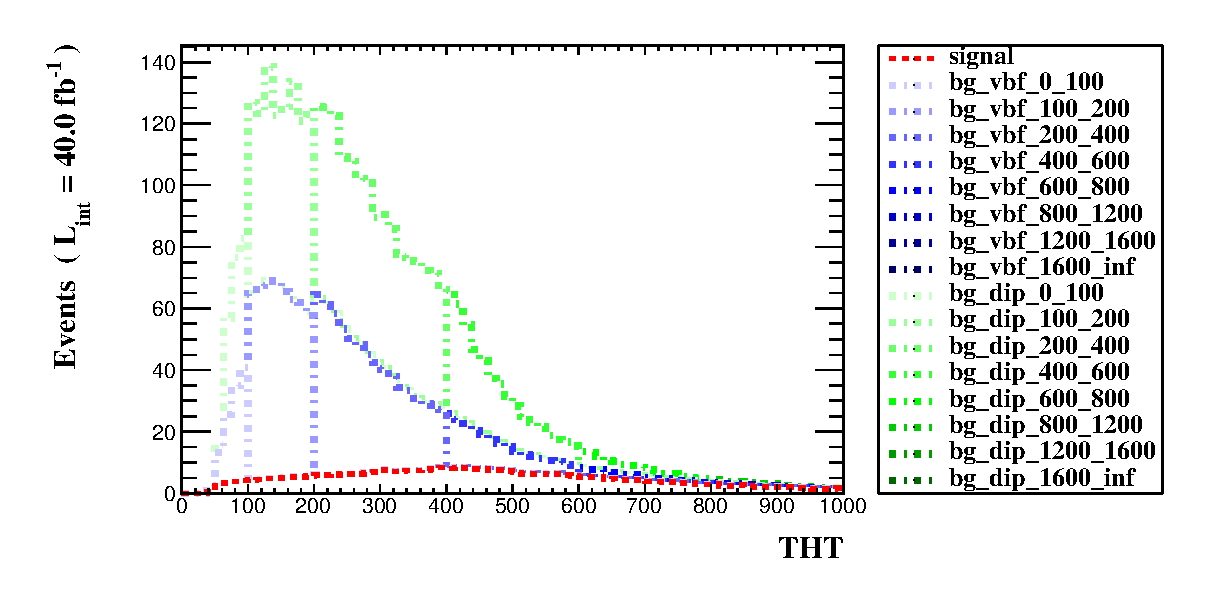
\includegraphics[scale=0.45]{selection_13.eps}\\
\caption{   }
  \end{center}
\end{figure}
      \newpage
\subsection{ Histogram 15}

\textbf{* Plot: MET}\\
   \begin{table}[H]
  \begin{center}
    \begin{tabular}{|m{23.0mm}|m{23.0mm}|m{18.0mm}|m{19.0mm}|m{19.0mm}|m{19.0mm}|m{19.0mm}|}
      \hline
      {\cellcolor{yellow}         Dataset}& {\cellcolor{yellow}         Integral}& {\cellcolor{yellow}         Entries per event}& {\cellcolor{yellow}         Mean}& {\cellcolor{yellow}         RMS}& {\cellcolor{yellow}         \% underflow}& {\cellcolor{yellow}         \% overflow}\\
      \hline
      {\cellcolor{white}         signal}& {\cellcolor{white}         405}& {\cellcolor{white}         1.0}& {\cellcolor{white}         8.08519e-09}& {\cellcolor{white}         1.046e-08}& {\cellcolor{green}         0.0}& {\cellcolor{green}         0.0}\\
      \hline
      {\cellcolor{white}         bg\_vbf\_0\_100}& {\cellcolor{white}         102}& {\cellcolor{white}         1.0}& {\cellcolor{white}         6.19944e-10}& {\cellcolor{white}         4.643e-10}& {\cellcolor{green}         0.0}& {\cellcolor{green}         0.0}\\
      \hline
      {\cellcolor{white}         bg\_vbf\_100\_200}& {\cellcolor{white}         477}& {\cellcolor{white}         1.0}& {\cellcolor{white}         1.03193e-09}& {\cellcolor{white}         1.184e-09}& {\cellcolor{green}         0.0}& {\cellcolor{green}         0.0}\\
      \hline
      {\cellcolor{white}         bg\_vbf\_200\_400}& {\cellcolor{white}         573}& {\cellcolor{white}         1.0}& {\cellcolor{white}         3.36658e-09}& {\cellcolor{white}         2.26e-09}& {\cellcolor{green}         0.0}& {\cellcolor{green}         0.0}\\
      \hline
      {\cellcolor{white}         bg\_vbf\_400\_600}& {\cellcolor{white}         136}& {\cellcolor{white}         1.0}& {\cellcolor{white}         4.57136e-09}& {\cellcolor{white}         2.627e-09}& {\cellcolor{green}         0.0}& {\cellcolor{green}         0.0}\\
      \hline
      {\cellcolor{white}         bg\_vbf\_600\_800}& {\cellcolor{white}         23.8}& {\cellcolor{white}         1.0}& {\cellcolor{white}         4.96532e-09}& {\cellcolor{white}         2.759e-09}& {\cellcolor{green}         0.0}& {\cellcolor{green}         0.0}\\
      \hline
      {\cellcolor{white}         bg\_vbf\_800\_1200}& {\cellcolor{white}         6.04}& {\cellcolor{white}         1.0}& {\cellcolor{white}         5.29507e-09}& {\cellcolor{white}         3.266e-09}& {\cellcolor{green}         0.0}& {\cellcolor{green}         0.0}\\
      \hline
      {\cellcolor{white}         bg\_vbf\_1200\_1600}& {\cellcolor{white}         0.337}& {\cellcolor{white}         1.0}& {\cellcolor{white}         7.57578e-09}& {\cellcolor{white}         9.664e-09}& {\cellcolor{green}         0.0}& {\cellcolor{green}         0.0}\\
      \hline
      {\cellcolor{white}         bg\_vbf\_1600\_inf}& {\cellcolor{white}         0.0252}& {\cellcolor{white}         1.0}& {\cellcolor{white}         1.17343e-08}& {\cellcolor{white}         1.543e-08}& {\cellcolor{green}         0.0}& {\cellcolor{green}         0.0}\\
      \hline
      {\cellcolor{white}         bg\_dip\_0\_100}& {\cellcolor{white}         117}& {\cellcolor{white}         1.0}& {\cellcolor{white}         7.65424e-10}& {\cellcolor{white}         5.853e-10}& {\cellcolor{green}         0.0}& {\cellcolor{green}         0.0}\\
      \hline
      {\cellcolor{white}         bg\_dip\_100\_200}& {\cellcolor{white}         496}& {\cellcolor{white}         1.0}& {\cellcolor{white}         1.18704e-09}& {\cellcolor{white}         1.387e-09}& {\cellcolor{green}         0.0}& {\cellcolor{green}         0.0}\\
      \hline
      {\cellcolor{white}         bg\_dip\_200\_400}& {\cellcolor{white}         814}& {\cellcolor{white}         1.0}& {\cellcolor{white}         3.50088e-09}& {\cellcolor{white}         2.275e-09}& {\cellcolor{green}         0.0}& {\cellcolor{green}         0.0}\\
      \hline
      {\cellcolor{white}         bg\_dip\_400\_600}& {\cellcolor{white}         292}& {\cellcolor{white}         1.0}& {\cellcolor{white}         4.46119e-09}& {\cellcolor{white}         2.584e-09}& {\cellcolor{green}         0.0}& {\cellcolor{green}         0.0}\\
      \hline
      {\cellcolor{white}         bg\_dip\_600\_800}& {\cellcolor{white}         44.6}& {\cellcolor{white}         1.0}& {\cellcolor{white}         4.86013e-09}& {\cellcolor{white}         2.677e-09}& {\cellcolor{green}         0.0}& {\cellcolor{green}         0.0}\\
      \hline
      {\cellcolor{white}         bg\_dip\_800\_1200}& {\cellcolor{white}         10.9}& {\cellcolor{white}         1.0}& {\cellcolor{white}         5.19487e-09}& {\cellcolor{white}         4.117e-09}& {\cellcolor{green}         0.0}& {\cellcolor{green}         0.0}\\
      \hline
      {\cellcolor{white}         bg\_dip\_1200\_1600}& {\cellcolor{white}         0.675}& {\cellcolor{white}         1.0}& {\cellcolor{white}         8.45939e-09}& {\cellcolor{white}         1.179e-08}& {\cellcolor{green}         0.0}& {\cellcolor{green}         0.0}\\
      \hline
      {\cellcolor{white}         bg\_dip\_1600\_inf}& {\cellcolor{white}         0.0437}& {\cellcolor{white}         1.0}& {\cellcolor{white}         1.08698e-08}& {\cellcolor{white}         1.476e-08}& {\cellcolor{green}         0.0}& {\cellcolor{green}         0.0}\\
\hline
    \end{tabular}
  \end{center}
\end{table}

\begin{figure}[H]
  \begin{center}
    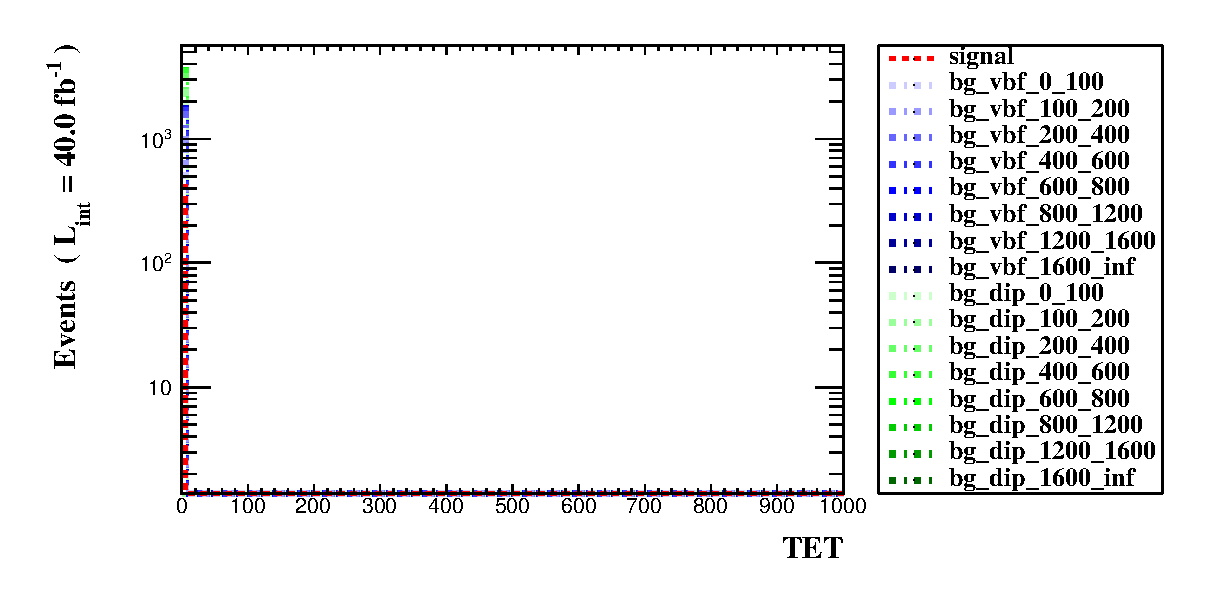
\includegraphics[scale=0.45]{selection_14.eps}\\
\caption{   }
  \end{center}
\end{figure}
      \newpage
\subsection{ Histogram 16}

\textbf{* Plot: TET}\\
   \begin{table}[H]
  \begin{center}
    \begin{tabular}{|m{23.0mm}|m{23.0mm}|m{18.0mm}|m{19.0mm}|m{19.0mm}|m{19.0mm}|m{19.0mm}|}
      \hline
      {\cellcolor{yellow}         Dataset}& {\cellcolor{yellow}         Integral}& {\cellcolor{yellow}         Entries per event}& {\cellcolor{yellow}         Mean}& {\cellcolor{yellow}         RMS}& {\cellcolor{yellow}         \% underflow}& {\cellcolor{yellow}         \% overflow}\\
      \hline
      {\cellcolor{white}         signal}& {\cellcolor{white}         405}& {\cellcolor{white}         1.0}& {\cellcolor{white}         1462.16}& {\cellcolor{white}         772.4}& {\cellcolor{red}         0.0}& {\cellcolor{red}         69.3}\\
      \hline
      {\cellcolor{white}         bg\_vbf\_0\_100}& {\cellcolor{white}         102}& {\cellcolor{white}         1.0}& {\cellcolor{white}         137.744}& {\cellcolor{white}         35.69}& {\cellcolor{green}         0.0}& {\cellcolor{green}         0.0}\\
      \hline
      {\cellcolor{white}         bg\_vbf\_100\_200}& {\cellcolor{white}         477}& {\cellcolor{white}         1.0}& {\cellcolor{white}         223.583}& {\cellcolor{white}         59.29}& {\cellcolor{green}         0.0}& {\cellcolor{green}         0.01051}\\
      \hline
      {\cellcolor{white}         bg\_vbf\_200\_400}& {\cellcolor{white}         573}& {\cellcolor{white}         1.0}& {\cellcolor{white}         387.623}& {\cellcolor{white}         105.1}& {\cellcolor{green}         0.0}& {\cellcolor{green}         0.08151}\\
      \hline
      {\cellcolor{white}         bg\_vbf\_400\_600}& {\cellcolor{white}         136}& {\cellcolor{white}         1.0}& {\cellcolor{white}         624.846}& {\cellcolor{white}         145.1}& {\cellcolor{green}         0.0}& {\cellcolor{green}         2.447}\\
      \hline
      {\cellcolor{white}         bg\_vbf\_600\_800}& {\cellcolor{white}         23.8}& {\cellcolor{white}         1.0}& {\cellcolor{white}         875.421}& {\cellcolor{white}         196.4}& {\cellcolor{red}         0.0}& {\cellcolor{red}         20.92}\\
      \hline
      {\cellcolor{white}         bg\_vbf\_800\_1200}& {\cellcolor{white}         6.04}& {\cellcolor{white}         1.0}& {\cellcolor{white}         1161.19}& {\cellcolor{white}         277.5}& {\cellcolor{red}         0.0}& {\cellcolor{red}         66.39}\\
      \hline
      {\cellcolor{white}         bg\_vbf\_1200\_1600}& {\cellcolor{white}         0.337}& {\cellcolor{white}         1.0}& {\cellcolor{white}         1641.82}& {\cellcolor{white}         397.8}& {\cellcolor{red}         0.0}& {\cellcolor{red}         100.0}\\
      \hline
      {\cellcolor{white}         bg\_vbf\_1600\_inf}& {\cellcolor{white}         0.0252}& {\cellcolor{white}         1.0}& {\cellcolor{white}         2198.57}& {\cellcolor{white}         636.7}& {\cellcolor{red}         0.0}& {\cellcolor{red}         100.0}\\
      \hline
      {\cellcolor{white}         bg\_dip\_0\_100}& {\cellcolor{white}         117}& {\cellcolor{white}         1.0}& {\cellcolor{white}         142.783}& {\cellcolor{white}         39.01}& {\cellcolor{green}         0.0}& {\cellcolor{green}         0.0}\\
      \hline
      {\cellcolor{white}         bg\_dip\_100\_200}& {\cellcolor{white}         496}& {\cellcolor{white}         1.0}& {\cellcolor{white}         228.006}& {\cellcolor{white}         64.22}& {\cellcolor{green}         0.0}& {\cellcolor{green}         0.0}\\
      \hline
      {\cellcolor{white}         bg\_dip\_200\_400}& {\cellcolor{white}         814}& {\cellcolor{white}         1.0}& {\cellcolor{white}         393.387}& {\cellcolor{white}         108.5}& {\cellcolor{green}         0.0}& {\cellcolor{green}         0.05657}\\
      \hline
      {\cellcolor{white}         bg\_dip\_400\_600}& {\cellcolor{white}         292}& {\cellcolor{white}         1.0}& {\cellcolor{white}         597.663}& {\cellcolor{white}         143.1}& {\cellcolor{green}         0.0}& {\cellcolor{green}         2.599}\\
      \hline
      {\cellcolor{white}         bg\_dip\_600\_800}& {\cellcolor{white}         44.6}& {\cellcolor{white}         1.0}& {\cellcolor{white}         847.17}& {\cellcolor{white}         201.6}& {\cellcolor{red}         0.0}& {\cellcolor{red}         15.68}\\
      \hline
      {\cellcolor{white}         bg\_dip\_800\_1200}& {\cellcolor{white}         10.9}& {\cellcolor{white}         1.0}& {\cellcolor{white}         1152.29}& {\cellcolor{white}         315.5}& {\cellcolor{red}         0.0}& {\cellcolor{red}         58.66}\\
      \hline
      {\cellcolor{white}         bg\_dip\_1200\_1600}& {\cellcolor{white}         0.675}& {\cellcolor{white}         1.0}& {\cellcolor{white}         1627.82}& {\cellcolor{white}         477.4}& {\cellcolor{red}         0.0}& {\cellcolor{red}         100.0}\\
      \hline
      {\cellcolor{white}         bg\_dip\_1600\_inf}& {\cellcolor{white}         0.0437}& {\cellcolor{white}         1.0}& {\cellcolor{white}         2198.72}& {\cellcolor{white}         744.6}& {\cellcolor{red}         0.0}& {\cellcolor{red}         100.0}\\
\hline
    \end{tabular}
  \end{center}
\end{table}

\begin{figure}[H]
  \begin{center}
    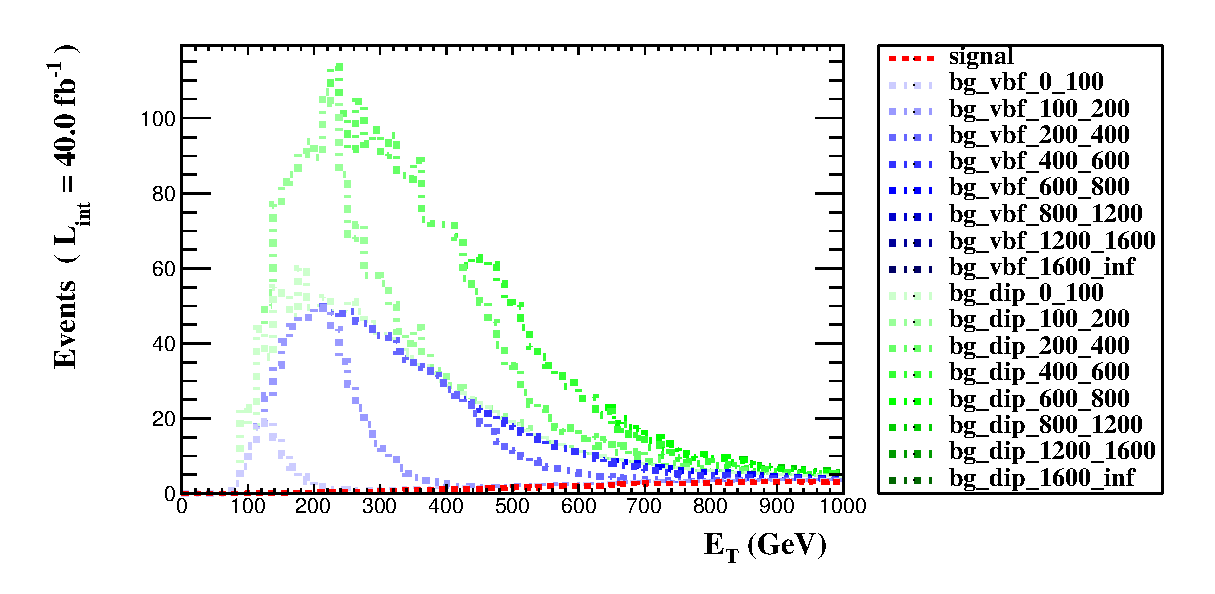
\includegraphics[scale=0.45]{selection_15.eps}\\
\caption{   }
  \end{center}
\end{figure}
      % -----------------------------------------------------------------------------
%                                SECTION Summary                                
% -----------------------------------------------------------------------------
\newpage
\section{ Summary}

\subsection{Cut-flow charts}

\begin{itemize}
  \item How to compare signal (S) and background (B): \textcolor{blue}{S/\-sqrt(S+B)} .
   \item Object definition selections are indicated in cyan.  \item Reject and select are indicated by 'REJ' and 'SEL' respectively
\end{itemize}
\begin{table}[H]
  \begin{center}
    \begin{tabular}{|m{36.0mm}|m{36.0mm}|m{36.0mm}|m{33.0mm}|}
      \hline
      {\cellcolor{yellow}        Cuts}& {\cellcolor{yellow}         Signal (S)}& {\cellcolor{yellow}         Background (B)}& {\cellcolor{yellow}         S vs B}\\
      \hline
      {\cellcolor{white}         Initial (no cut)}& {\cellcolor{white}         4094.08 +/\-- 1.13}& {\cellcolor{white}         4113516 +/\-- 4877}& {\cellcolor{white}         2.01760 +/\-- 0.00132}\\
      \hline
      {\cellcolor{white} SEL: sdETA ( jets[1] jets[2] ) > 3.6 and M ( jets[}& {\cellcolor{white}         405.3 +/\-- 19.1}& {\cellcolor{white}         3098.1 +/\-- 54.7}& {\cellcolor{white}         6.847 +/\-- 0.309}\\
\hline
    \end{tabular}
  \end{center}
\end{table}

\end{document}
